\documentclass[journal]{IEEEtran}
\usepackage[T1]{fontenc}
\usepackage{amsmath,amssymb,bm}
\usepackage{booktabs,multirow,array,longtable}
\usepackage{graphicx}
\usepackage{tikz}
\usetikzlibrary{arrows.meta,decorations.pathreplacing,positioning}
\usepackage{cite}
\usepackage[hidelinks]{hyperref}
\graphicspath{{./}}
\newcommand{\Tr}{\operatorname{Tr}}
\newcommand{\RMSE}{\mathrm{RMSE}}
\newcommand{\cRMSE}{\mathrm{cRMSE}}
\setlength{\emergencystretch}{2em}
\newcommand{\fitcol}[1]{\resizebox{\ifdim\width>\columnwidth\columnwidth\else\width\fi}{!}{#1}}

\begin{document}

\title{Hardware-Aware Design and Layout Selection in Quantum Reservoir Computing for Insurance Claims Forecasting}

\author{[Author names]%
\thanks{[Affiliations, corresponding author and e-mail.]}}

\markboth{IEEE Transactions on Quantum Engineering}{Hardware-aware quantum reservoir forecasting of insurance claims}

\maketitle

\begin{abstract}
We ask two questions about a gate-based quantum reservoir computer (QRC) applied to next-day forecasting of motor-insurance claim counts: whether it forecasts competitively, and whether it can be designed and placed on a noisy processor so that its predictions survive the transfer from simulation. The reservoir has four injection and two memory qubits evolving under a Trotterized Ising Hamiltonian with transverse and memory-local fields, and a ridge readout trained in noiseless simulation. Hardware-native interaction graphs, Hamiltonian parameters, readout observables and temporal windows were chosen with five explicit selection rules and calibrated noisy simulation, giving five frozen candidates. On 232 held-out test days the ideal reservoirs reach a root-mean-square error (RMSE) of 5.66--6.12 claims/day, within the bootstrap uncertainty of ridge regression (5.36) for four of five candidates and better than gradient-boosted trees (6.28). We then executed each candidate 3--5 times on IBM Kingston under three layout policies run in parallel: a hardware-aware (HA) search ending in a training-only processor probe, a uniformly random native embedding and the Qiskit level-1 mapping, for 63 full evaluations. HA gave lower forecast error than Qiskit in 21 of 21 rounds. Against random layouts the typical error was similar, but random placement produced the four largest distortions of the study (13--35 claims/day), each on a layout containing a coupler that calibration data reported as degraded or broken; HA never exceeded 7.6. Most of the hardware distortion is a constant level shift, and the HA probe predicts it before deployment (leave-one-out $R^2=0.74$).
\end{abstract}

\begin{IEEEkeywords}
Hardware-aware quantum computing, insurance forecasting, NISQ devices, quantum reservoir computing, qubit mapping, time-series forecasting.
\end{IEEEkeywords}

\section{Introduction}
\IEEEPARstart{C}{urrent} quantum processors have tens to hundreds of qubits, gate errors around $10^{-3}$, coherence times of a few hundred microseconds and calibration data that change from hour to hour \cite{Preskill2018NISQ,Bharti2022NISQ,Klimov2018Fluctuations}. Algorithms that ask for long coherent evolution or deep, trained circuits are difficult to run reliably on such machines. Reservoir computing is attractive under these constraints because the dynamical system is fixed and only a linear readout is trained \cite{Jaeger2004ESN,Lukosevicius2009RC}. In quantum reservoir computing (QRC) the reservoir is a driven many-body quantum system and the readout acts on measured expectation values \cite{Fujii2017QRC,Mujal2021Review}. Because model fitting does not require gradient-based optimization of quantum-circuit parameters, the barren-plateau and gradient-estimation issues associated with variational quantum algorithms do not arise. The difficulty is instead shifted from simulation-based training to QPU transfer. The readout is fitted to features computed in simulation, whereas the processor returns observables altered by decoherence, gate and readout errors, and finite sampling. Whether a QRC forecaster preserves its simulated behavior on hardware therefore depends both on the reservoir design and on the physical qubits on which it is executed \cite{Chen2020Noisy,Murali2019NoiseAdaptive,Tannu2019NotAll,Niu2020HardwareAware,Nation2023Mapomatic}.

We study this question in the context of next-day insurance claim-count forecasting, a standard actuarial time-series problem in which claim frequency is modelled relative to portfolio exposure and calendar effects \cite{Harvey1989Claims,Wuthrich2023Actuarial}. Our dataset contains four and a half years of daily motor third-party-liability property-damage claims from a commercial insurer, together with the number of active policies and calendar information. During the observation period the insured portfolio grows substantially, so the evaluation period includes exposure levels beyond those seen during training. The data are partitioned chronologically into training, validation, and held-out test periods, with all feature selection, model tuning, and candidate selection performed without access to the test targets. This setting therefore allows us to examine two complementary research questions:

\paragraph{Forecasting performance}
Can the QRC architecture forecast insurance claims competitively with classical statistical, recurrent, and reservoir models when all models use the same inputs and are frozen before testing?

\paragraph{Simulation-to-QPU transfer}
Can the architecture be designed and placed on real NISQ hardware in a systematic way, so that its forecasts transfer reliably from simulation to the processor?

\begin{figure*}[t]
\centering
\resizebox{\textwidth}{!}{%% ---- fig_workflow.tex
% Overview of the study: problem mapping, logical design and hardware deployment.
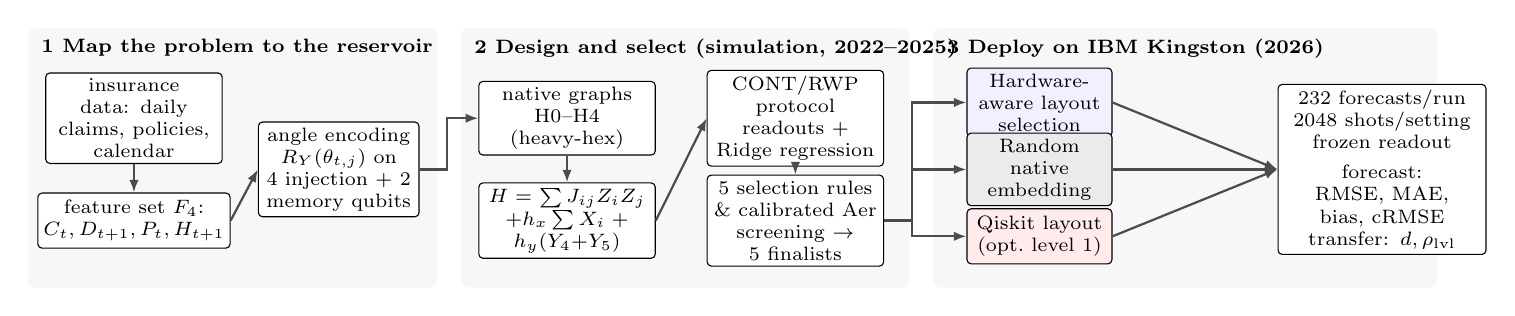
\begin{tikzpicture}[
  font=\scriptsize,
  box/.style={draw, rounded corners=1.5pt, align=center, minimum height=7mm, inner sep=2pt, fill=white},
  stage/.style={draw=black!25, rounded corners=3pt, fill=black!3},
  arr/.style={-{Latex[length=1.6mm]}, thick, black!70},
  lab/.style={font=\scriptsize\bfseries, anchor=north west}]
% stage frames
\fill[black!3, rounded corners=3pt] (0,0) rectangle (5.2,3.3);
\fill[black!3, rounded corners=3pt] (5.5,0) rectangle (11.2,3.3);
\fill[black!3, rounded corners=3pt] (11.5,0) rectangle (17.9,3.3);
\node[lab] at (0.05,3.28) {1 Map the problem to the reservoir};
\node[lab] at (5.55,3.28) {2 Design and select (simulation, 2022--2025)};
\node[lab] at (11.55,3.28) {3 Deploy on IBM Kingston (2026)};
% stage 1
\node[box, text width=21mm] (data) at (1.35,2.15) {insurance data: daily claims, policies, calendar};
\node[box, text width=23mm] (feat) at (1.35,0.85) {feature set $F_4$:\\ $C_t,D_{t+1},P_t,H_{t+1}$};
\node[box, text width=19mm] (enc) at (3.95,1.5) {angle encoding\\ $R_Y(\theta_{t,j})$ on\\ 4 injection + 2 memory qubits};
\draw[arr] (data) -- (feat);
\draw[arr] (feat.east) -- (enc.west);
% stage 2
\node[box, text width=21mm] (topo) at (6.85,2.15) {native graphs\\ H0--H4 (heavy-hex)};
\node[box, text width=21mm] (ham) at (6.85,0.85) {$H=\sum J_{ij}Z_iZ_j$\\ $+h_x\sum X_i+h_y(Y_4{+}Y_5)$};
\node[box, text width=21mm] (rules) at (9.75,2.15) {CONT/RWP protocol readouts + Ridge regression};
\node[box, text width=21mm] (aer) at (9.75,0.85) {5 selection rules \& calibrated Aer\\ screening $\to$ 5 finalists};
\draw[arr] (enc.east) -- ++(0.35,0) |- (topo.west);
\draw[arr] (topo) -- (ham);
\draw[arr] (ham.east) -- (rules.west);
\draw[arr] (rules) -- (aer);
% stage 3
\node[box, text width=17mm, fill=blue!6] (ha) at (12.85,2.35) {Hardware-aware layout selection};
\node[box, text width=17mm, fill=black!8] (rnd) at (12.85,1.5) {Random native\\ embedding};
\node[box, text width=17mm, fill=red!8] (qk) at (12.85,0.65) {Qiskit layout\\ (opt.\ level 1)};
\node[box, text width=25mm] (qpu) at (17.2,1.5)
{232 forecasts/run\\
2048 shots/setting\\
frozen readout\\[1mm]
forecast: RMSE, MAE,\\ bias, cRMSE\\
transfer: $d,\rho_{\rm lvl}$};
\draw[arr] (aer.east) -- ++(0.35,0) |- (rnd.west);
\draw[arr] (aer.east) ++(0.35,0) |- (ha.west);
\draw[arr] (aer.east) ++(0.35,0) |- (qk.west);
\draw[arr] (ha.east) -- (qpu.west);
\draw[arr] (rnd.east) -- (qpu.west);
\draw[arr] (qk.east) -- (qpu.west);
\end{tikzpicture}
}
\caption{High-level workflow from forecasting inputs to reservoir design, candidate selection, and QPU evaluation under three layout policies.}
\label{fig:workflow}
\end{figure*}

To answer these two questions, we propose a complete problem-to-processor workflow consisting of three stages, summarized in Fig.~\ref{fig:workflow}.
In Stage~1, the insurance forecasting problem is reduced to the four-input feature set $F_4$, and the inputs are encoded into a six-qubit reservoir with four injection and two memory qubits. 
Stage~2 performs the logical and hardware-aware reservoir design using training and validation data only: the native interaction graph, Hamiltonian parameters, temporal protocol, observable set, and ridge readout are selected, after which five candidates are frozen following the five selection rules and calibrated noisy-simulation screening. 
Stage~3 evaluates these unchanged candidates on the held-out 2026 period. Each candidate is executed on IBM Kingston under three physical-layout policies: hardware-aware, random native, and Qiskit level~1, and is assessed with both conventional forecasting metrics and the simulation-to-QPU transfer distortion. 
The two research questions are examined separately throughout the study. A reservoir that forecasts well in simulation need not be the one whose predictions are preserved most faithfully on hardware, while a hardware perturbation can occasionally reduce target error through bias compensation without representing a better transferred model.

The main contributions of this work are as follows.
\begin{itemize}

\item \emph{A reproducible hardware-aware QRC workflow.}
We provide a fully reproducible pipeline, including the selection rules, intermediate candidate sets, calibration-aware screening, and frozen final configurations. The workflow is summarized in Fig.~\ref{fig:workflow}, and the implementation and recorded outputs are available in the public repository.\footnote{\url{https://github.com/rusnakrenata/qrc_insurance}}

underprediction of the higher portfolio level.


\item \emph{A repeated hardware comparison of physical-layout policies.}
We execute the five frozen candidates in 21 paired rounds on IBM Kingston, giving 63 complete hardware evaluations under hardware-aware, random-native, and Qiskit level-1 mappings. Hardware-aware placement yields lower forecast error than Qiskit in all 21 rounds and limits transfer distortion to at most 7.6 claims/day, while random placement produces four catastrophic distortions of 13--35 claims/day on layouts containing degraded or broken couplers.

\item \emph{An observable-level explanation and pre-deployment estimate of QPU transfer error.}
Hardware transfer is dominated by systematic shifts in the measured reservoir features rather than by random forecast fluctuations. The level-shift component exceeds half of the total distortion in 44 of 63 runs; for one candidate, a single memory-qubit correlator contributes about +5.3 claims/day to the shift. A short probe using training inputs predicts the subsequent hardware distortion with leave-one-round-out $R^2=0.74$, whereas calibrated noisy simulation underestimates its magnitude by a median factor of 4.2.

\end{itemize}
We do not claim a quantum advantage. Ridge regression remains the most accurate model on this dataset, which is largely driven by linear exposure and calendar effects.

The paper is organized as follows. Section~II reviews related work. Section~III states the forecasting problem, data, objectives and metrics. Section~IV defines the reservoir. Section~V describes how the hardware candidates were designed and selected, and Section~VI the hardware execution protocol and classical baselines. Section~VII reports results for both objectives, Section~VIII discusses them, and Section~IX concludes. The appendices list classical configurations, all hardware runs and reproducibility details.

\section{Related Work}
\subsection{Forecasting insurance claims}
Claim counts are classically modelled with Poisson and negative-binomial generalized linear models, often with exposure as an offset \cite{Nelder1972GLM,Cameron2013Count,Wuthrich2023Actuarial}. Structural time-series models treat aggregate claims as a random sum with dynamic components \cite{Harvey1989Claims}. Tree ensembles and neural networks are now common in pricing and frequency modelling \cite{Henckaerts2021Boosting,Wuthrich2023Actuarial}, but comparative studies find that the advantage over count regression depends on the dataset and the metric \cite{Alomair2024Count}. Quantum methods have been proposed for risk analysis and pricing in finance and insurance \cite{Egger2020Finance}, and a recent study used QRC features with boosting for motor-insurance claim severity in noise-free simulation \cite{Tamturk2026Insurance}. We are not aware of QRC applied to claim-count forecasting on quantum hardware.

\subsection{Classical reservoir computing and recurrent models}
Echo state networks train only a linear map from a fixed random recurrent network \cite{Jaeger2004ESN,Lukosevicius2009RC}; their memory is usually quantified by the linear memory capacity \cite{Jaeger2002STM}. Dambre et al.\ generalized it to an information-processing capacity measured with orthogonal polynomial targets: a reservoir with $N$ linearly independent features, driven by independent inputs, has a total capacity of at most $N$, which it divides between linear recall of past inputs and nonlinear functions of them \cite{Dambre2012Capacity}. Linear memory therefore shows only part of what a reservoir computes. Physical reservoirs replace the network with a dynamical substrate \cite{Tanaka2019Physical}. Recurrent neural networks and gated recurrent units learn the dynamics as well \cite{Elman1990RNN,Cho2014GRU}. These models are the natural classical counterparts of a QRC and are included as baselines.

\subsection{Quantum reservoir computing}
Fujii and Nakajima introduced QRC with disordered transverse-field Ising ensembles and showed that the exponentially large state space supplies nonlinear features with fading memory \cite{Fujii2017QRC}. Spatial multiplexing of several small reservoirs increases computational power without enlarging any one of them \cite{Nakajima2019Multiplexing}, and quantum reservoir processing applies the idea to quantum inputs \cite{Ghosh2019Processing}. For time-series prediction, memory depends strongly on the input interval and on coupling disorder \cite{Kutvonen2020Optimizing}, and reservoir performance tracks the dynamical phase of the underlying spin model, with the ergodic regime favourable for processing \cite{MartinezPena2021Phase}. Measurement is a central limitation. Projective measurement destroys the state, so temporal QRC either uses weak measurement or restarts the dynamics and replays the recent input history for every output (rewinding), at a cost that grows with the history length \cite{Mujal2023Measurements}. Finite sampling adds noise that degrades forecasts unless training accounts for it \cite{Ahmed2025FiniteSampling}. Quantum extreme learning machines, the memoryless limit of QRC, are bounded in expressivity by the measured observables \cite{Innocenti2023QELM}. Dissipation and device noise can supply fading memory rather than only degrade it \cite{Suzuki2022Natural,Kubota2023Noise,Sannia2024Dissipation,Ricci2026Damping}; this is a property of the reservoir as a computer, not a guarantee that a readout trained in simulation will tolerate a processor's noise.

\subsection{Gate-based and hybrid reservoirs}
Not all QRCs are Hamiltonian quench dynamics. Several studies build the reservoir from angle-encoding rotations and fixed entangling layers. Wudarski \emph{et al.} use random input projections fed into single-qubit rotations followed by CNOT rings and a ridge readout on single-qubit and correlator expectation values \cite{Wudarski2023Hybrid}. The recurrence-free QRC of Ahmed \emph{et al.} removes the recurrent unitary, applies fully entangling CNOT layers and a random unitary, and moves memory into a classical leaky integrator \cite{Ahmed2024RecurrenceFree}. Hybrid reservoirs of this kind have modelled thermal convection \cite{Pfeffer2022Convection}. Their entanglement pattern is chosen for expressivity rather than for a hardware coupling map, and memory is often carried classically. Our reservoir sits between the two families: it is a Trotterized Ising Hamiltonian, as in Hamiltonian QRC, but implemented as a gate circuit whose interaction graph is chosen to embed natively in the processor, with a quantum memory register reset only at window boundaries.

\subsection{QRC on hardware and in applications}
Chen \emph{et al.} ran temporal QRC on IBM processors and showed that noise can be absorbed when the readout is trained on hardware data \cite{Chen2020Noisy}. Suzuki \emph{et al.} used the natural noise of a superconducting device as the reservoir \cite{Suzuki2022Natural}. Recent work forecasts chaotic dynamics with reservoir networks on NISQ hardware \cite{Connerty2026Hardware}, multivariate series with rewind windows on an IBM Heron device \cite{Hamhoum2025Multivariate}, and realized volatility in simulation \cite{Li2026Volatility}; large reservoirs have also been realized on analog neutral-atom hardware \cite{Kornjaca2024Analog}. Table~\ref{tab:related} compares the closest works. In most hardware studies the physical placement is left to the compiler, and the readout is either retrained on hardware data or the reported comparison is between simulation and one hardware run. The question of which placement policy preserves a frozen forecaster, and how reproducibly, has not been tested with repeated paired runs.

\begin{table*}[t]
\centering
\caption{Closest QRC Studies Compared With This Work}
\label{tab:related}
\footnotesize
\setlength{\tabcolsep}{3.5pt}
\begin{tabular}{@{}p{2.3cm}p{2.4cm}p{2.9cm}p{1.1cm}p{2.1cm}p{1.8cm}p{2.0cm}p{1.7cm}@{}}
\toprule
Work & Input encoding & Reservoir dynamics & Qubits & Memory & Readout & Hardware & Task \\
\midrule
Fujii and Nakajima \cite{Fujii2017QRC} & state of one input qubit & disordered transverse-field Ising quench & 5--7 & quantum, continuous & linear & none & benchmark series \\
Kutvonen \emph{et al.} \cite{Kutvonen2020Optimizing} & input qubit state & fully connected Ising ($XX$+$Z$ field) & $\le 7$ & quantum, continuous & linear & none & stock index \\
Chen \emph{et al.} \cite{Chen2020Noisy} & gate rotations & dissipative gate circuit & small & quantum & linear, trained on hardware & IBM & temporal tasks \\
Wudarski \emph{et al.} \cite{Wudarski2023Hybrid} & random projection, $U_3$ angles & CNOT rings & 6--8 & classical feedback & ridge & OQC Lucy (proof of concept) & chaotic systems \\
Ahmed \emph{et al.} \cite{Ahmed2024RecurrenceFree} & rotation angles & CNOT entangling + random unitary & 9--11 & classical leaky integrator & ridge & none & chaotic, extreme events \\
Hamhoum \emph{et al.} \cite{Hamhoum2025Multivariate} & $R_Y$ on injection qubits & Trotterized $XX$ Ising + field & 6--15 & memory qubits, rewind window & ridge & IBM Heron & Lorenz-63, ENSO \\
Tamturk \emph{et al.} \cite{Tamturk2026Insurance} & data features & QRC feature map & -- & -- & boosting & none & claim severity \\
This work & $R_Y$ angles, clipped and soft-saturated & Trotterized $ZZ$ Ising, $X$ field, memory $Y$ field, native graphs & 6 & 2 memory qubits, reset-window replay & ridge, frozen & IBM Kingston, 63 runs; IQM probe & daily claim counts \\
\bottomrule
\end{tabular}
\end{table*}

\subsection{Hardware-aware mapping and calibration variability}
Mapping logical qubits to physical ones is a compilation problem with a long history \cite{Siraichi2018Allocation,Li2019SABRE}. Noise-adaptive and variability-aware mappings use calibration data to avoid weak qubits and couplers \cite{Murali2019NoiseAdaptive,Tannu2019NotAll,Niu2020HardwareAware}, and mapomatic scores candidate layouts by predicted fidelity \cite{Nation2023Mapomatic}. For circuits whose interaction graph already embeds natively, the problem reduces to initial placement without routing \cite{Steinberg2022Assignment}; Qiskit's VF2Layout solves this with subgraph isomorphism \cite{Cordella2004VF2,JavadiAbhari2024Qiskit}. Benchmarks of circuit transformation show large gaps between compiler heuristics and near-optimal costs \cite{Li2025QKNOB}. All these methods optimize a circuit-level figure of merit derived from calibration data, which fluctuate on time scales of minutes to hours \cite{Klimov2018Fluctuations,Burnett2019Decoherence,Proctor2020Drift}. A forecaster cares about something else: how far its predictions move. We therefore compare a layout criterion defined on the forecaster's output with an error-rate-based compiler mapping and with random placement.

\paragraph*{What is new here} QRC, rewinding, Trotterized Ising reservoirs, calibration-aware mapping and block bootstrapping are established. The contributions of this paper are their combination into a selection procedure for a hardware-deployable forecaster, the paired multi-round hardware comparison of placement policies, and the analysis of how and when the forecasts fail on the processor.

\section{Problem Formulation and Objectives}
\subsection{Forecasting task and data}
Let $C_t$ be the number of property-damage claims reported on day $t$ and $P_t$ the number of active policies on that day. The target is $y_t=C_{t+1}$. At forecast origin $t$ the inputs are $C_t$, $P_t$, the weekday $D_{t+1}\in\{0,\dots,6\}$ of the target day and a Slovak public-holiday indicator $H_{t+1}$. All four are known at the time of the forecast; the calendar of day $t+1$ is fixed in advance. The forecast origins run from 1~January~2022 to 19~August~2026 (1692 days). They are split chronologically into training (2022--2024, 1095 days), validation (2025, 365 days) and test (1~January--20~August~2026, 232 days) periods. Observed 2026 claims enter later forecasts as inputs, but no model parameter is updated during the test period.

Table~\ref{tab:setup} summarizes the setup and Fig.~\ref{fig:data} shows the series. The portfolio grew from about 90\,000 to 222\,000 policies. Mean daily claims rose from 8.86 in training to 14.89 in the test period, while claim frequency stayed between 0.076 and 0.085 claims per thousand policies per day (Table~\ref{tab:encoding}). Most of the growth in claims is portfolio growth.

\begin{figure}[t]
\centering
\includegraphics[width=\columnwidth]{fig_data}
\caption{Daily claim counts (gray) with 28-day mean, the level above which the claims angle saturates (dashed), and the number of active policies. Dotted lines separate training, validation (2025) and test (2026) periods.}
\label{fig:data}
\end{figure}

\begin{table}[t]
\centering
\caption{Study Setup}
\label{tab:setup}
\footnotesize
\setlength{\tabcolsep}{3pt}
\begin{tabular}{@{}p{2.1cm}p{6.1cm}@{}}
\toprule
Item & Setting \\
\midrule
Target & next-day claim count $y_t=C_{t+1}$ \\
Inputs ($F_4$) & $C_t$, $P_t$, weekday $D_{t+1}$, holiday $H_{t+1}$ \\
Splits & train 2022--24 ($n$=1095), validation 2025 (365), test 2026 (232) \\
Normalization & $z$-scores with training mean and SD; quantum angles in (\ref{eq:enc}) \\
Model selection & 5-fold expanding-window CV on 2022--24; one configuration per model selected on 2025; 2026 scored once \\
Classical models & Ridge, Poisson and NB2 GLMs, ESN, vanilla RNN, GRU, XGBoost (squared, Poisson), naive baselines \\
Quantum model & 6 qubits (4 injection, 2 memory), Trotterized Ising reservoir, ridge readout \\
Hardware & IBM Kingston (Heron r2, 156 qubits, heavy-hex), CZ native gate \\
Execution & 2048 shots per setting, 2 settings, 464 circuits per run, opt.\ level 1, no routing \\
Layout policies & hardware-aware (HA), random native, Qiskit \\
Metrics & RMSE, MAE, bias, cRMSE, transfer distortion $d$, level-shift share (Table~\ref{tab:metrics}) \\
\bottomrule
\end{tabular}
\end{table}

\subsection{Choice of predictors}
\label{sec:predictors}
The insurer's daily export contains claim counts by type (total, property damage, injury, loss of profit), the number of active policies, policy-age counts and shares, the share of policies held by legal entities, the mean vehicle age and calendar flags. The target is the property-damage count, which equals the total minus injury and loss-of-profit claims. Every encoded input costs qubits, gates and circuit time, so the inputs were fixed by an analysis of the training period alone, before any model was tuned. The total count was dropped because it contains $C_t$; injury and loss-of-profit counts correlate weakly with $C_{t+1}$ ($r=0.02$ and $0.11$). The portfolio-composition variables track the portfolio size: on the training period the legal-entity share correlates with $P_t$ at $-0.96$, the share of policies older than four years at $-0.92$ and the mean vehicle age at $0.69$, and all are built from monthly snapshots. A ranking by correlation with the target would have selected several copies of the same growth trend.

Table~\ref{tab:predictors} summarizes the evidence for the four remaining candidates. Mutual information (MI) measures any statistical dependence, not only linear dependence, and is compared with its distribution under 500 random permutations of the target. $\Delta R^2$ is the increase in explained variance when a variable is added to a linear model that already contains the listed controls. The weekday alone accounts for 24\,\% of the target variance (one-way ANOVA, $\eta^2=0.237$). Holidays are rare (44 training days) but halve the claim count, and they add explained variance beyond the weekday that no within-weekday shuffle of the holiday labels reproduced ($10^4$ shuffles). The current count $C_t$ is almost uncorrelated with $C_{t+1}$ ($r=0.10$), yet its MI exceeds the permutation threshold; the dependence is nonlinear, which is the kind of structure a reservoir is meant to expose. The policy count adds 4.7 percentage points of explained variance beyond the calendar but only 0.7 once a linear time trend is included, so its contribution is mostly the portfolio growth. The target autocorrelation peaks at multiples of seven days ($\rho_7=0.31$, $\rho_{28}=0.29$), but beyond the calendar, policies and $C_t$ the weekly lags add less than 0.1 percentage points of explained variance. Only $C_{t-1}$ adds more (0.7 points), and that short history is what the memory of the reservoir and of the recurrent models supplies, so no explicit lag vector was built. The candidates are not redundant: the largest pairwise correlation is 0.21, every variance inflation factor (VIF) is at most 2.0, and weekday and holiday are nearly independent (Cram\'er's $V=0.077$).

Three nested input sets followed: $F_2=(C_t,D_{t+1})$, $F_3=F_2\cup\{P_t\}$ and $F_4=F_3\cup\{H_{t+1}\}$. Before the classical benchmark, the three sets were compared with the linear models only: ridge regression (penalty chosen by cross-validation on 2022--2024) and Poisson and NB2 GLMs, each fitted on 2022--2024 and scored on 2025. Adding $P_t$ lowered the 2025 RMSE from 6.30--6.32 to 4.94--5.01 claims/day in all three models, and adding $H_{t+1}$ lowered it by a further 0.06--0.14, to 4.87--4.88. $F_4$ was therefore fixed for all later stages; the cross-validated searches of the ESN, RNN, GRU and XGBoost, which were free to choose among $F_2$--$F_4$, selected it as well (Appendix~A).

\begin{table}[t]
\centering
\caption{Screening of Candidate Predictors on the Training Period (2022--2024)}
\label{tab:predictors}
\footnotesize
\setlength{\tabcolsep}{2.5pt}
\begin{tabular}{@{}lccp{4.15cm}@{}}
\toprule
Input & $r$ & MI ($p$) & Additional evidence \\
\midrule
$D_{t+1}$ & $-$0.38$^{a}$ & 0.117 (0.002) & weekday explains 24\,\% of variance; Sat/Sun means 6.5/5.3 vs 9.5--10.5 \\
$H_{t+1}$ & $-$0.25 & 0.040 (0.002) & mean 4.0 vs 9.1; $\Delta R^2=0.069$ beyond weekday, $p<10^{-4}$ \\
$C_t$ & 0.10 & 0.048 (0.022) & weak linear, significant nonlinear dependence \\
$P_t$ & 0.21 & 0.023 (0.15) & $\Delta R^2=0.047$ beyond calendar; 0.007 beyond calendar and trend \\
\bottomrule
\end{tabular}

\smallskip
\parbox{\columnwidth}{\scriptsize $r$: Pearson correlation with $C_{t+1}$. MI in nats, $p$ from 500 target permutations. $^{a}$Weekday is categorical; the sign of $r$ is not meaningful.}
\end{table}

\subsection{Objectives}
\emph{Objective~1 (forecasting).} Determine whether, and under what conditions, the QRC forecasts next-day claims competitively with classical models that use the same inputs and the same chronological protocol.

\emph{Objective~2 (hardware-aware design).} Determine whether systematic, hardware-aware choice of interaction graph, parameters, circuit configuration and physical layout preserves the forecaster's predictions on a noisy processor, and compare this with the compiler's default mapping and with random placement.

\subsection{Metrics}
With $e_t=\hat y_t-y_t$ over the $n=232$ test days, we report the root-mean-square error $\RMSE=(n^{-1}\sum_t e_t^2)^{1/2}$, the mean absolute error, and the bias $\bar e=n^{-1}\sum_t e_t$ (positive values over-predict). The centered RMSE removes the bias,
\begin{equation}
\RMSE^2=\bar e^{\,2}+\cRMSE^2,\qquad \cRMSE^2=\tfrac1n\textstyle\sum_t (e_t-\bar e)^2 ,
\label{eq:crmse}
\end{equation}
so it measures how well a model follows day-to-day variation regardless of level.

For a hardware run we compare the processor prediction $\hat y^Q_t$ with the ideal prediction $\hat y^I_t$ of the same frozen model, $\delta_t=\hat y^Q_t-\hat y^I_t$. The \emph{transfer distortion} is $d=(n^{-1}\sum_t\delta_t^2)^{1/2}$, in claims per day. It splits into a constant part and a fluctuating part, $d^2=\bar\delta^{\,2}+\mathrm{Var}_t(\delta_t)$; the \emph{level-shift share} is $\rho_{\rm lvl}=\bar\delta^{\,2}/d^2$. A share close to one means that the processor moves every forecast by roughly the same amount. The forecast error on hardware then satisfies
\begin{equation}
\mathrm{MSE}^Q=\mathrm{MSE}^I+d^2+\tfrac2n\textstyle\sum_t e^I_t\,\delta_t ,
\label{eq:interaction}
\end{equation}
where $e^I_t$ is the ideal error. The last term is negative when the hardware perturbation points against the ideal error, which is how a distorted forecast can score better than its own ideal model. Table~\ref{tab:metrics} lists the quantities used in the paper.

\begin{table}[t]
\centering
\caption{Metrics and Symbols}
\label{tab:metrics}
\footnotesize
\setlength{\tabcolsep}{3pt}
\begin{tabular}{@{}p{1.6cm}p{6.6cm}@{}}
\toprule
Symbol & Meaning \\
\midrule
RMSE, MAE & forecast error against observed claims (claims/day) \\
Bias $\bar e$ & mean forecast error; $>0$ over-predicts \\
cRMSE & RMSE after removing the bias, eq.~(\ref{eq:crmse}) \\
$\Delta$ & difference in RMSE between two models on the same days; negative favours the first \\
$d$ & transfer distortion: RMS of hardware minus ideal prediction \\
$\bar\delta$ & level shift: mean of hardware minus ideal prediction \\
$\rho_{\rm lvl}$ & level-shift share $\bar\delta^2/d^2$ \\
Daily gap & $|\delta_t|$ for one day; summarized by its median per run \\
$\eta_j,\zeta_j$ & contraction and offset of observable $j$: $z^Q_{t,j}\approx\eta_j z^I_{t,j}+\zeta_j$ \\
$L(\ell)$ & workload error proxy of layout $\ell$, eq.~(\ref{eq:proxy}) \\
Round & one paired execution of HA, random and Qiskit layouts for one candidate \\
\bottomrule
\end{tabular}
\end{table}

\subsection{Uncertainty}
Forecast errors on consecutive days are correlated, so we never treat days as independent. Differences between two models on the same test days are assessed with a circular block bootstrap \cite{Politis1992Circular} using 14-day blocks and 4000 resamples; blocks of 7 and 28 days were used as a sensitivity check. Intervals are not adjusted for multiple comparisons. Hardware runs differ in layout, calibration and execution time, so the run is the unit of replication. For layout comparisons we resample rounds within each candidate and dates in 14-day blocks (two-level bootstrap), and report the number of rounds in which one policy is better together with an exact sign test. We do not report significance for quantities that lack replication.

\section{Quantum Reservoir Model}
\subsection{Registers and input injection}
The reservoir has six qubits (Fig.~\ref{fig:reservoir}a). Qubits $q_0,\dots,q_3$ are injection qubits carrying $C_t$, $D_{t+1}$, $P_t$ and $H_{t+1}$; $q_4$ and $q_5$ form the memory register $M$. At each input step the injection register is reset and prepared as $\rho_I(\bm\theta_t)=\bigotimes_{j=0}^{3}R_Y(\theta_{t,j})|0\rangle\langle 0|R_Y(\theta_{t,j})^\dagger$, while the memory register keeps its state. With $z_C$ and $z_P$ the claims and policy counts standardized on the training period, the angles are
\begin{equation}
\bm\theta_t=\Bigl(a\,\tfrac{\mathrm{clip}(z_C,-3,3)}{3},\;\tfrac{2\pi D_{t+1}}{7},\;a\,\tfrac{z_P}{3+|z_P|},\;\pi H_{t+1}\Bigr).
\label{eq:enc}
\end{equation}
The weekday is periodic and is mapped to a full rotation. The encoding scale $a$ keeps the claims and exposure angles in the near-linear region of the qubit response. Exposure is soft-saturated rather than clipped: during design, clipping at three standard deviations mapped every 2025 and 2026 exposure value to the same angle, whereas the soft-sign map preserved their ordering. The claims angle is clipped; how often this happens in each period is reported in Section~VII-A.

\subsection{Hamiltonian}
The six qubits evolve under
\begin{equation}
H=\sum_{(i,j)\in E}J_{ij}Z_iZ_j+h_x\sum_{i=0}^{5}X_i+h_y\,(Y_4+Y_5),
\label{eq:ham}
\end{equation}
where $E$ is a logical coupling graph with five edges (Section~V). The $ZZ$ couplings create correlations and entanglement along the graph and carry information from the injection register into memory. The transverse field $h_x$ does not commute with the couplings; it rotates populations and turns the $Z$-basis encoding into dynamics. Without it, the evolution would only add phases in the computational basis.

The $Z$--$X$ Ising model has a global parity symmetry $\prod_i X_i$, is real in the computational basis, and on a chain maps to free fermions. The $R_Y$ injection breaks the parity at every input step, but between injections the evolution keeps it. A field along a third axis breaks these properties; tilted or mixed-field Ising chains are the standard nonintegrable variants with ergodic dynamics \cite{Banuls2011Thermalization,Kim2013Ballistic}, and reservoir memory has been linked to the dynamical regime of the spin model \cite{MartinezPena2021Phase}. We restricted the $Y$ field to the memory qubits so that it enriches the memory dynamics without changing the interaction graph or the injection map, and treated $h_y$ as a search parameter, with $h_y=0$ always available. In a paired comparison with otherwise identical search budgets, adding the field raised the memory capacity of H2, H3 and H4 by 2--43\,\% and changed cross-validated RMSE by at most 0.07 claims/day in either direction. All five final candidates have $h_y\neq0$, but the experiments do not show that the $Y$ term is necessary for forecasting, and we make no such claim.

\subsection{Trotterization and temporal protocols}
Each input step applies a first-order product formula with $r$ slices,
\begin{equation}
U=\Bigl[\prod_{(i,j)\in E}\!e^{-iJ_{ij}Z_iZ_j\tau}\prod_{i}e^{-ih_xX_i\tau}\!\prod_{m=4,5}\!e^{-ih_yY_m\tau}\Bigr]^r\!,
\label{eq:trotter}
\end{equation}
with $\tau=\Delta t/r$ and $\Delta t=1.6$. Changing $r$ at fixed couplings changes every slice angle, so the Trotter depth is a design parameter of the reservoir rather than only an approximation level, and $r$ was optimized together with $J$, $h_x$, $h_y$ and the readout penalty. After evolution the memory state is $\rho_M(t)=\Tr_I[U(\rho_I(\bm\theta_t)\otimes\rho_M(t-1))U^\dagger]$; on hardware the partial trace is a mid-circuit reset of the injection qubits.

A projective measurement destroys the reservoir state, so features for every forecast cannot be read from one long evolution. We use reset-window replay (RWP): for forecast origin $t$, the memory starts in $|00\rangle$ and the last $W$ inputs $\bm\theta_{t-W+1},\dots,\bm\theta_t$ are injected in sequence, after which all qubits are measured \cite{Mujal2023Measurements}. Two candidates were designed as continuous reservoirs, in which memory is carried through the whole chronology; for hardware they are deployed with a replay window longer than their stable washout time (Section~V-E).

\subsection{Measurement and readout}
The measured features are expectation values $z_{t,j}=\Tr(O_j\rho_t)$ of single-qubit $X_j$ and $Z_j$ operators on the injection qubits and, for two candidates, the memory correlator $Y_4X_5$. They are estimated from two measurement settings, one in a mixed $X$/$Y$ basis and one in the $Z$ basis. The forecast is
\begin{equation}
\hat y_t=b+\mathbf w^\top\mathbf z_t,\qquad (Z_s^\top Z_s+\lambda I)\bm\beta=Z_s^\top(\mathbf y-\bar y),
\label{eq:readout}
\end{equation}
where $Z_s$ holds training features standardized to zero mean and unit variance, $\mathbf w$ is $\bm\beta$ rescaled to raw units and $b$ is unpenalized \cite{Hoerl1970Ridge}. The readout is fitted once on noiseless features of the training period and used unchanged in noisy simulation and on hardware. An independent density-matrix implementation written for this paper reproduces all stored ideal features to $3\times10^{-14}$ and all readout weights to $3\times10^{-10}$.

\begin{figure*}[t]
\centering
\resizebox{\textwidth}{!}{%% ---- fig_reservoir.tex
% (a) one reset-window-replay step; (b) logical coupling graphs.
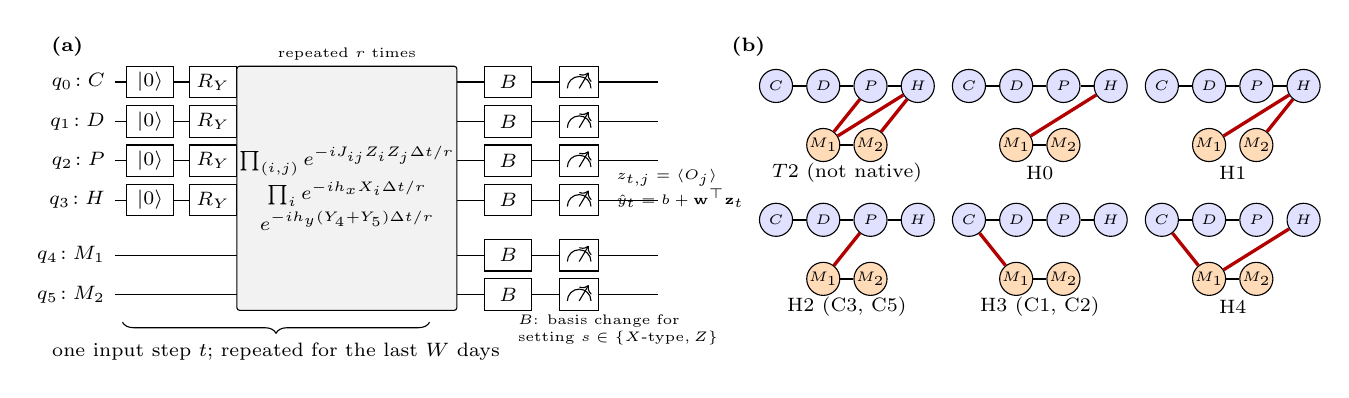
\begin{tikzpicture}[font=\scriptsize,
  gate/.style={draw, fill=white, minimum height=4mm, minimum width=6mm, inner sep=1pt},
  big/.style={draw, fill=black!5, rounded corners=1pt, align=center, inner sep=1pt}]
\node[font=\scriptsize\bfseries] at (-0.6,3.25) {(a)};
\foreach \y/\n in {2.8/$q_0\!:C$,2.3/$q_1\!:D$,1.8/$q_2\!:P$,1.3/$q_3\!:H$,0.6/$q_4\!:M_1$,0.1/$q_5\!:M_2$} {
  \node[anchor=east] at (0,\y) {\n};
  \draw (0,\y) -- (6.9,\y);
}
\node[anchor=east, font=\tiny] at (0,0.95) {};
\foreach \y in {2.8,2.3,1.8,1.3} {
  \node[gate] at (0.45,\y) {$|0\rangle$};
  \node[gate] at (1.25,\y) {$R_Y$};
}
\node[big, minimum height=31mm, minimum width=19mm] at (2.95,1.45) {$\prod_{(i,j)}e^{-iJ_{ij}Z_iZ_j\Delta t/r}$\\[1pt] $\prod_i e^{-ih_xX_i\Delta t/r}$\\[1pt] $e^{-ih_y(Y_4+Y_5)\Delta t/r}$};
\node[font=\tiny] at (2.95,3.15) {repeated $r$ times};
\draw[decorate, decoration={brace, amplitude=4pt, mirror}] (0.1,-0.25) -- (4.0,-0.25)
  node[midway, below=4pt, align=center] {one input step $t$; repeated for the last $W$ days};
\foreach \y in {2.8,2.3,1.8,1.3,0.6,0.1} { \node[gate] at (5.0,\y) {$B$}; }
\foreach \y in {2.8,2.3,1.8,1.3,0.6,0.1} {
  \node[draw, fill=white, minimum height=4mm, minimum width=5mm] (m\y) at (5.9,\y) {};
  \draw (5.75,\y-0.08) arc (180:0:0.15);
  \draw[->] (5.9,\y-0.08) -- (6.02,\y+0.12);
}
\node[align=left, anchor=west, font=\tiny] at (5.0,-0.35) {$B$: basis change for\\ setting $s\in\{X\text{-type},Z\}$};
\node[font=\tiny, align=left, anchor=west] at (6.25,1.45) {$z_{t,j}=\langle O_j\rangle$\\ $\hat y_t=b+\mathbf w^\top\mathbf z_t$};
% (b) graphs
\begin{scope}[xshift=8.4cm, yshift=0.15cm,
  inj/.style={circle,draw,fill=blue!12,inner sep=0pt,minimum size=4.2mm,font=\tiny},
  mem/.style={circle,draw,fill=orange!28,inner sep=0pt,minimum size=4.2mm,font=\tiny},
  e/.style={thick}, b/.style={very thick, red!70!black}]
\node[font=\scriptsize\bfseries] at (-0.35,3.1) {(b)};
\newcommand{\nodesat}[2]{%
  \begin{scope}[shift={(#1,#2)}]
  \node[inj] (0) at (0,0.75) {$C$}; \node[inj] (1) at (0.6,0.75) {$D$};
  \node[inj] (2) at (1.2,0.75) {$P$}; \node[inj] (3) at (1.8,0.75) {$H$};
  \node[mem] (4) at (0.6,0) {$M_1$}; \node[mem] (5) at (1.2,0) {$M_2$};
  \end{scope}}
\nodesat{0}{1.85}
\draw[e] (0)--(1) (1)--(2) (2)--(3) (4)--(5); \draw[b] (2)--(4) (3)--(4) (3)--(5);
\node at (0.9,1.5) {$T2$ (not native)};
\nodesat{2.45}{1.85}
\draw[e] (0)--(1) (1)--(2) (2)--(3) (4)--(5); \draw[b] (3)--(4);
\node at (3.35,1.5) {H0};
\nodesat{4.9}{1.85}
\draw[e] (0)--(1) (1)--(2) (2)--(3); \draw[b] (3)--(4) (3)--(5);
\node at (5.8,1.5) {H1};
\nodesat{0}{0.15}
\draw[e] (0)--(1) (1)--(2) (2)--(3) (4)--(5); \draw[b] (2)--(4);
\node at (0.9,-0.2) {H2 (C3, C5)};
\nodesat{2.45}{0.15}
\draw[e] (0)--(1) (1)--(2) (2)--(3) (4)--(5); \draw[b] (0)--(4);
\node at (3.35,-0.2) {H3 (C1, C2)};
\nodesat{4.9}{0.15}
\draw[e] (0)--(1) (1)--(2) (4)--(5); \draw[b] (0)--(4) (3)--(4);
\node at (5.8,-0.2) {H4};
\end{scope}
\end{tikzpicture}
}
\caption{(a) One reset-window-replay step: injection qubits are reset and encoded with $R_Y(\theta_{t,j})$, the six qubits evolve under $r$ Trotter slices of (\ref{eq:ham}), and after $W$ steps all qubits are measured in one of two settings. (b) Logical coupling graphs; red edges connect the injection and memory registers. $T2$ maximized memory in simulation but contains triangles absent from heavy-hex hardware; H0--H4 are five-edge trees that embed without SWAP gates.}
\label{fig:reservoir}
\end{figure*}

\section{From Logical Design to Five Hardware Candidates}
The design work preceded any use of 2026 data and is summarized here as five stages (stage 2 in Fig.~\ref{fig:workflow}). All selection decisions used the training period, with 2025 used only for ranking.


\subsection{Problem mapping}
The input set $F_4$ chosen in Section~\ref{sec:predictors} was confirmed by the classical searches: every temporal family (ESN, vanilla RNN, GRU) selected $F_4$ over $F_2$ and $F_3$ in chronological cross-validation, so $F_4$ was frozen before the quantum search. The number of memory qubits (one to four), the policy encoding and the replay window (1--28 days) were then chosen in noiseless simulation; two memory qubits and the encoding in (\ref{eq:enc}) were retained.

\subsection{Hardware-native interaction graphs}
The first memory-optimized reservoir used a seven-edge graph $T2$ (Fig.~\ref{fig:reservoir}b) with several paths into the memory register. It reached a channel-averaged memory capacity $\mathrm{MC}_{\rm ch}=1.27$ (delays 1--20, finite-sample corrected \cite{Dambre2012Capacity}). IBM Heron processors use a heavy-hex lattice of maximum degree three without triangles \cite{Chamberland2020HeavyHex}, and an exhaustive search found no native embedding of $T2$ on any of the three processors profiled (IBM Fez, Kingston and Marrakesh). Rather than route a non-native graph, we designed five six-vertex trees of maximum degree three that differ in how information reaches memory: a chain with one boundary edge (H0), a holiday fan-out into both memory qubits without a memory--memory edge (H1), a policy branch into an interacting memory pair (H2), a reordered chain with the claims qubit at the memory boundary (H3) and a memory hub (H4). On Kingston they have 1072 (H0, H3), 516 (H1, H4) and 264 (H2) native embeddings.

\subsection{Setting the Hamiltonian parameters}
Couplings cannot be transplanted from $T2$, because an edge means something different on each graph. Each graph therefore received the same budget: 32 coupling vectors (28 Latin-hypercube samples in $J_{ij}\in[-2,2]$ and four uniform anchors) and 20 coordinate refinements, with $a=0.75$, $h_x=0.5$, $r=2$ fixed. H2, H3 and H4 retained 97\,\%, 90\,\% and 79\,\% of the memory capacity of $T2$; H0 and H1 retained 2\,\%. An injection--memory edge feeding an interacting memory pair is needed; a memory edge alone (H0) or direct fan-out alone (H1) is not. H2 and H3 found the same coupling vector on different edges, yet H2 kept 8\,\% more memory, so the placement of couplings matters as well as their values. Because H1 forecast well with almost no memory, no graph was discarded at this stage.

The $Y$ field was then added and the parameters $(J,h_x,h_y,\lambda)$ re-optimized for each $r\in\{1,2,3\}$: 15 dynamics seeds (graph and $h_y$ value), each with three observable sets, searched over $h_x\in\{0.25,0.5,0.75\}$ and global coupling scales $\{0.5,1,1.5\}$ with local refinement and reselection of $\lambda$. The best cross-validated depth was $r=3$ in 32 of 45 branches. Process fidelity of the Trotter circuit was recorded but not optimized; the most accurate continuous reservoir (H4, $r=3$) had a process fidelity of only 0.37.

Observable sets were checked for shot resolvability. In an early hardware test, the holiday observable $X_3$ varied with a standard deviation of 0.017 on training data, below the 0.031 shot noise at 1024 shots, and its readout weight raised the hardware RMSE to about 39 claims/day; removing it brought the error to about 5.5. Observable sets are therefore chosen per candidate.

\subsection{Five selection rules and noisy screening}
Different objectives favour different reservoirs, so we did not combine them into one score. Rules 1--4 were applied to every graph under continuous and replay operation: (R1) minimum mean cross-validated RMSE; (R2) maximum delayed-input memory, defined below; (R3) measurement robustness, requiring every feature's shot noise at 1024 shots to be below its natural variation and then minimizing the forecast shot noise $(\sum_j (w_j/\sigma_j)^2(1-\mu_j^2)/N)^{1/2}$; (R4) the cheapest circuit within one standard error of the best cross-validated RMSE, ranked by SWAP count, CZ count, measurement settings, depth and duration. Rule R5 selects the processor and physical region from calibration data. The rule map contained 33 unique reservoirs (17 continuous, 16 replay). All compiled without SWAP gates on the three Heron processors. One Trotter slice costs ten CZ gates, so a two-setting replay feature vector costs about $20rW$ CZ gates.

\emph{Delayed-input memory (R2).} Memory was treated as a design objective of its own, not as a proxy for forecasting accuracy; several good forecasters found during development used replay windows of one or two days. Following the linear memory capacity of reservoir computing \cite{Jaeger2002STM,Dambre2012Capacity}, the four encoded input channels of 2022--2025 were permuted independently, which keeps their marginal distributions and removes all temporal structure. The reservoir was driven by this probe in its own protocol (continuous or replay) and a ridge readout ($\lambda=10^{-6}$) on the 18 one-body Pauli expectations was trained on 2022--2024 endpoints to recover the input $u_j(t-k)$ of channel $j$, $k$ steps back. With $\hat u_{j,k}$ the prediction on the 365 endpoints of 2025,
\begin{equation}
\mathrm{MC}_{j,k}=\max\!\Big(\mathrm{Corr}^2\big(u_j(t-k),\hat u_{j,k}(t)\big)-\tfrac{1}{N_{\rm val}-1},\,0\Big),
\label{eq:mc}
\end{equation}
where the subtracted term is the expected squared correlation of unrelated sequences \cite{Dambre2012Capacity}. Rule R2 maximized the channel average $\mathrm{MC}_{\rm ch}^{1:20}=\frac14\sum_{j}\sum_{k=1}^{20}\mathrm{MC}_{j,k}$, averaged over five probe seeds for replay reservoirs. The upper limit $k=20$ is a fixed diagnostic horizon, not a measured memory length. R2 measures linear delayed-input memory only; the nonlinear capacity of the finalists was measured afterwards (Section~\ref{sec:capacity}) and played no part in the selection. Memory capacity differs from washout: it asks how much of a past input can be read linearly from the current features, whereas washout asks how quickly the reservoir forgets an arbitrary initial state. Continuous reservoirs therefore also had to reach a stable washout to qualify under R2; replay reservoirs restart from $|00\rangle$ at every endpoint and have no such condition. With replay the memory is bounded by construction, because the features at endpoint $t$ depend only on inputs $t-W+1,\dots,t$, so delays $k\ge W$ are unreachable \cite{Mujal2023Measurements}.

All 33 reservoirs were then simulated with a Kingston-calibrated gate and thermal-relaxation noise model at $(r,N)\in\{(2,1024),(3,512),(3,1024),(3,2048),(4,512)\}$, three repetitions each. Calibrated noise improved 17 and degraded 16 candidates, so it was not treated as beneficial in general. The Pareto front in validation RMSE, CZ count per feature vector and shots contained nine operating points, all from H3 and H2 replay and H2 and H0 continuous reservoirs. No H1 or H4 point was non-dominated: the best H4 point (replay, $W=14$, RMSE 4.99 at 840 CZ) is dominated by an H3 point (4.98 at 120 CZ).

\subsection{The five candidates}
The finalists were chosen to answer different questions rather than as the five lowest errors (Table~\ref{tab:cand}). C1 (H3, R1/R3) is the accuracy leader. C2 (H3, R4) halves its circuit cost. C3 (H2, R3) is the shallowest measurement-robust replay reservoir. C4 (H0, R4) is a cheap continuous reservoir on the front, and C5 (H2, R2) is the memory-first design. A remote job cannot keep a quantum state between separately submitted daily forecasts, so the continuous candidates were replayed with windows above their stable washout time (the number of steps after which both the trace distance between different initial memory states and the distance between their feature vectors stay below 0.01): $W=117$ for C4 and $W=64$ for C5. Their readouts remain the continuous-operation fits; the replayed ideal forecasts match continuous operation to within 0.003 RMSE. Readouts were finally refitted with fold-local standardization and frozen before any 2026 data were scored.

\begin{table}[t]
\centering
\caption{The Five Frozen Candidates}
\label{tab:cand}
\footnotesize
\setlength{\tabcolsep}{2.2pt}
\fitcol{%% ---- tables/tab_candidates.tex
\begin{tabular}{@{}lcccccccccccc@{}}
\toprule
& Graph & $W$ & $r$ & $a$ & $h_x$ & $h_y$ & $\lambda$ & $m$ & CV & 2025 & CZ & $t_{\rm c}$ ($\mu$s) \\
\midrule
C1 & H3 & 4 & 3 & 0.25 & 0.777 & $-$0.293 & $10^{-4}$ & 8 & 3.46 & 4.71 & 240 & 16 \\
C2 & H3 & 2 & 3 & 0.25 & 0.777 & $-$0.293 & $10^{-1}$ & 7 & 3.54 & 4.94 & 120 & 8 \\
C3 & H2 & 2 & 2 & 0.75 & 0.491 & +0.398 & $10^{2}$ & 7 & 3.62 & 5.06 & 80 & 8 \\
C4 & H0 & 117$^{*}$ & 4 & 0.75 & 0.580 & $-$0.694 & $10^{2}$ & 9 & 3.67 & 5.03 & 9360 & 499 \\
C5 & H2 & 64$^{*}$ & 2 & 0.75 & 0.491 & +0.398 & $10^{2}$ & 8 & 3.59 & 4.98 & 2560 & 233 \\
\bottomrule
\end{tabular}
}
\vspace{2pt}
\parbox{\columnwidth}{\footnotesize $W$: replay window ($^{*}$continuous design deployed with replay); $r$: Trotter slices; $a$: encoding scale; $m$: number of observables; CV: cross-validated RMSE on 2022--24; 2025: validation RMSE (claims/day); CZ: gates per feature vector (two settings); $t_{\rm c}$: scheduled circuit duration of the longer setting on Kingston.}
\end{table}

\section{Hardware Execution and Baselines}
\subsection{Three layout policies}
For each candidate and round, one shared preparation step fixed the ideal reference and a calibration snapshot of IBM Kingston, from which a gate and thermal-relaxation noise model was exported. Three independent workers then selected their layouts and executed the same frozen model.
\begin{itemize}
\item \emph{Hardware-aware (HA).} Enumerate native embeddings on the current coupling map; keep those that compile without routing; rank them by the workload error proxy
\begin{equation}
L(\ell)=-\sum_{g\in G_\ell}\log(1-\epsilon_g)-\sum_{q\in M_\ell}\log(1-\epsilon^{\rm RO}_q),
\label{eq:proxy}
\end{equation}
summed over every gate and measurement of the compiled workload; simulate the six best layouts with the calibrated noise model on 20 training dates at 64 shots; run the two with the smallest prediction distortion on the processor at 100 evenly spaced training dates and 256 shots; deploy the one with the smaller measured distortion. No 2026 label enters the selection.
\item \emph{Random native.} Shuffle all native embeddings that avoid qubits flagged as faulty and take the first that compiles without routing. No error rates are used.
\item \emph{Qiskit.} Transpile a representative circuit at optimization level~1 \cite{JavadiAbhari2024Qiskit}, extract the initial mapping and recompile with routing disabled. The recorded transpiler traces show VF2Layout for C1, C2, C3 and C5 and the trivial layout (qubits 0--5) for C4, whose chain graph embeds there directly.
\end{itemize}
All policies used 2048 shots per setting, optimization level~1 and two measurement settings, giving 464 circuits per evaluation of the 232 test days (C4 and C5 in three sequential jobs). Readout-error mitigation was not applied. The three evaluations of a round were submitted from separate processes at the same time and started executing a median of 21~minutes apart (at most 5~hours, for the chunked C4 and C5 jobs). IBM recalibrates on its own schedule, and the calibration changed between layout selection and execution in 40 of 63 runs, which we record but cannot control. The object of comparison is the choice of physical qubits, not the compiler's gate optimization, so all three policies share one optimization level. We checked offline whether a higher Qiskit level would have changed the baseline, using a saved Kingston calibration and one training date per candidate. Levels~2 and~3 select the initial layout with the same VF2Layout pass that level~1 used for C1, C2, C3 and C5, and the compiled circuits kept the same CZ count with durations within 2\,\%. Level~2 returned the level-1 qubits for these four candidates; level~3, which runs VF2Layout with a larger search budget, chose other qubits. For C4 both higher levels replaced the trivial layout with a VF2Layout placement. Since the selection algorithm is the same, we did not repeat the hardware comparison at levels~2 and~3.

Twenty-one complete rounds were executed between 7 and 11 October 2026: five for C1--C3 and three for C4 and C5. The same candidates had been run on the 2026 dates in an earlier exploratory campaign (2--5 October) that compared HA and Qiskit layouts only; that campaign led to the parallel three-policy protocol and to common settings for all candidates (2048 shots, six-layout HA pool). Reservoirs and readouts were frozen before any 2026 data were scored, and only the runs described here are reported. Two further folders were excluded before analysis, one empty preparation and one round in which an IBM API error stopped all three workers before execution. Appendix~B lists every run with its physical layout.

\subsection{Classical baselines}
The classical models use the same $F_4$ inputs and chronology, with the weekday entered as its sine and cosine. They cover the families an actuary would try first and the closest classical analogues of a QRC: ridge regression \cite{Hoerl1970Ridge}; Poisson and negative-binomial (NB2) GLMs with exposure as covariate or log offset \cite{Nelder1972GLM,Cameron2013Count}; an ESN \cite{Jaeger2004ESN}; a vanilla RNN and a GRU \cite{Elman1990RNN,Cho2014GRU}; and XGBoost with squared-error and Poisson objectives \cite{Chen2016XGBoost}, together with seasonal-naive, persistence and training-mean forecasts. Every classical family went through the same three steps. First, five-fold expanding-window cross-validation on 2022--2024 ranked its configurations, and the three with the lowest mean fold RMSE were kept; for the GLMs, which have no tuning parameters, the configurations were seven predefined exposure specifications. Second, the three were fitted on 2022--2024 and scored on 2025, and the one with the lowest 2025 RMSE was retained; the three naive forecasts were compared on 2025 directly. Third, only this configuration, still fitted on 2022--2024, was scored on 2026, once. Stochastic models were run with ten fixed seeds; both their 2025 score and their 2026 result are means over seeds, and no seed was selected. Appendix~A lists the cross-validated configurations, their 2025 scores and the selected one. The QRC readout has 7--9 coefficients, comparable to Ridge and the GLMs and far fewer than the recurrent networks.

\section{Results}
\subsection{Objective 1: forecasting performance}
Table~\ref{tab:forecast} and Fig.~\ref{fig:forecast} compare all models on the 232 test days. Ridge regression is the most accurate model (RMSE 5.36). The ideal reservoirs reach 5.66--6.12. For C1, C3, C4 and C5 the 95\,\% block-bootstrap interval of the difference to Ridge includes zero; C2 is worse by 0.76 [0.05, 1.43]. With 7-day blocks the interval for C3 just excludes zero, and with 28-day blocks the one for C2 just includes it; the other conclusions do not depend on the block length. All five ideal reservoirs are more accurate than XGBoost with squared loss, by 0.16--0.62 claims/day, with intervals excluding zero. The ESN (5.60) is ahead of all five. C4, C5 and C1 are slightly ahead of the GRU (5.76), C3 and C2 behind it; four of the five are ahead of the vanilla RNN (6.11), and all are ahead of the Poisson GLM and Poisson XGBoost.

\begin{table*}[t]
\centering
\caption{Forecast Accuracy on the 2026 Test Period (232 Days, Claims/Day)}
\label{tab:forecast}
\footnotesize
%% ---- tables/tab_forecast.tex
\begin{tabular}{@{}lccccc c@{}}
\toprule
Model & RMSE & MAE & Bias & cRMSE & $\Delta$ vs Ridge & $\Delta$ vs XGBoost (sq.) \\
\midrule
Ridge & 5.36 & 4.11 & +0.32 & 5.35 & +0.00 [+0.00, +0.00] & $-$0.92 [$-$1.63, $-$0.15] \\
NB2 GLM & 5.57 & 4.28 & +0.86 & 5.50 & +0.21 [$-$0.03, +0.46] & $-$0.71 [$-$1.54, +0.25] \\
ESN$^\dagger$ & 5.60 & 4.31 & +0.41 & 5.40 & +0.24 [+0.12, +0.35] & $-$0.68 [$-$1.32, +0.02] \\
GRU$^\dagger$ & 5.76 & 4.45 & $-$1.50 & 5.54 & +0.40 [$-$0.03, +0.80] & $-$0.52 [$-$0.89, $-$0.10] \\
Vanilla RNN$^\dagger$ & 6.11 & 4.71 & $-$2.15 & 5.56 & +0.75 [+0.23, +1.25] & $-$0.17 [$-$0.41, +0.09] \\
XGBoost (squared) & 6.28 & 4.83 & $-$3.67 & 5.10 & +0.92 [+0.16, +1.61] & +0.00 [+0.00, +0.00] \\
Poisson GLM & 6.47 & 5.06 & +2.93 & 5.76 & +1.10 [+0.43, +1.85] & +0.19 [$-$0.95, +1.56] \\
XGBoost (Poisson) & 6.63 & 5.14 & $-$4.29 & 5.05 & +1.27 [+0.44, +2.04] & +0.35 [+0.27, +0.42] \\
\midrule
C1, ideal & 5.76 & 4.36 & $-$2.80 & 5.03 & +0.39 [$-$0.30, +1.02] & $-$0.53 [$-$0.68, $-$0.36] \\
C1, QPU (HA)$^\ddagger$ & 6.36 & 5.08 & +1.72 & 5.31 & +1.00 [+0.72, +1.31] & +0.08 [$-$0.65, +0.87] \\
C2, ideal & 6.12 & 4.64 & $-$3.12 & 5.27 & +0.76 [+0.05, +1.43] & $-$0.16 [$-$0.28, $-$0.04] \\
C2, QPU (HA)$^\ddagger$ & 5.81 & 4.43 & $-$1.61 & 5.56 & +0.45 [$-$0.07, +0.92] & $-$0.47 [$-$0.76, $-$0.15] \\
C3, ideal & 5.94 & 4.47 & $-$2.62 & 5.33 & +0.58 [$-$0.08, +1.14] & $-$0.34 [$-$0.51, $-$0.17] \\
C3, QPU (HA)$^\ddagger$ & 5.75 & 4.38 & $-$1.37 & 5.50 & +0.39 [$-$0.08, +0.79] & $-$0.53 [$-$0.85, $-$0.20] \\
C4, ideal & 5.66 & 4.34 & $-$1.54 & 5.45 & +0.30 [$-$0.16, +0.69] & $-$0.62 [$-$0.97, $-$0.26] \\
C4, QPU (HA)$^\ddagger$ & 5.83 & 4.65 & +0.84 & 5.67 & +0.47 [+0.21, +0.72] & $-$0.45 [$-$1.13, +0.26] \\
C5, ideal & 5.75 & 4.32 & $-$2.16 & 5.33 & +0.39 [$-$0.16, +0.91] & $-$0.53 [$-$0.76, $-$0.29] \\
C5, QPU (HA)$^\ddagger$ & 5.72 & 4.49 & +0.69 & 5.60 & +0.35 [+0.10, +0.59] & $-$0.57 [$-$1.22, +0.14] \\
\bottomrule
\end{tabular}

\vspace{2pt}
\parbox{\textwidth}{\footnotesize $\Delta$: RMSE of the model minus RMSE of the reference, with 95\,\% circular-block bootstrap interval (14-day blocks). $^\dagger$Mean over ten seeds. $^\ddagger$Mean over the 3--5 IBM Kingston runs with HA layouts; hardware results are discussed in Section~VII-B.}
\end{table*}

\begin{figure}[t]
\centering
\includegraphics[width=\columnwidth]{fig_forecasting}
\caption{Test RMSE of classical models, ideal reservoirs and HA hardware runs. Open markers and bars show the error on the first and last 116 test days; the dashed line marks Ridge.}
\label{fig:forecast}
\end{figure}

The structure of the QRC error explains the ranking. Once the level is removed, the reservoirs follow daily variation as well as Ridge: cRMSE is 5.03 for C1 and 5.27--5.45 for the others, against 5.35 for Ridge. They lose on level. All five under-predict (bias $-1.5$ to $-3.1$), whereas Ridge, being linear in exposure, extrapolates the portfolio trend (bias $+0.32$). On the first 116 test days every ideal reservoir ties or beats Ridge (RMSE 5.07--5.35 against 5.36); on the last 116 days, when counts are highest, they fall behind (5.95--6.87 against 5.37). XGBoost shows the same pattern more strongly (bias $-3.67$), because trees cannot extrapolate either.

Table~\ref{tab:encoding} shows why. The claims angle saturates above $\bar C+3\sigma_C\approx20.9$ claims, which happened on 0.5\,\% of training days, 7.7\,\% of 2025 days and 16.4\,\% of 2026 days (21.6\,\% in the second half). The normalized exposure angle spanned $-0.30$ to $0.49$ in training and $0.65$ to $0.77$ in 2026, so the readout extrapolates along an input it never saw vary in that range. Claim frequency, by contrast, stayed between 0.076 and 0.085. As a diagnostic only, refitting the readout on 2022--2025 with unchanged features, encoding and $\lambda$ lowers the ideal 2026 RMSE to 5.28--5.54 (C1: 5.28), against 5.39 for Ridge refitted in the same way (Table~\ref{tab:refit}). The reservoir features carry the information; the frozen readout was anchored to a smaller portfolio.

\begin{table}[t]
\centering
\caption{Inputs Relative to the Training Range}
\label{tab:encoding}
\footnotesize
\setlength{\tabcolsep}{2.4pt}
\fitcol{%% ---- tables/tab_encoding.tex
\begin{tabular}{@{}lcccccc@{}}
\toprule
Period & $n$ & Mean $C$ & Clipped (\%) & Policies ($10^3$) & $\theta_P/a$ & Claims per $10^3$ pol. \\
\midrule
train 2022-24 & 1095 & 8.86 & 0.5 & 89.5--138.2 & $-$0.30--0.49 & 0.085 \\
validation 2025 & 365 & 12.71 & 7.7 & 138.3--170.7 & 0.49--0.65 & 0.082 \\
test 2026 first half & 116 & 13.51 & 11.2 & 170.8--186.8 & 0.65--0.70 & 0.076 \\
test 2026 second half & 116 & 16.37 & 21.6 & 187.0--221.8 & 0.70--0.77 & 0.081 \\
\bottomrule
\end{tabular}
}
\vspace{2pt}
\parbox{\columnwidth}{\footnotesize Clipped: share of days on which the claims angle saturates. $\theta_P/a$: exposure angle divided by the encoding scale.}
\end{table}

\begin{table}[t]
\centering
\caption{Ideal Reservoirs With the Readout Refitted Through 2025}
\label{tab:refit}
\footnotesize
\setlength{\tabcolsep}{3pt}
\fitcol{%% ---- tables/tab_refit.tex
\begin{tabular}{@{}lccccc@{}}
\toprule
 & \multicolumn{3}{c}{Readout fitted on 2022--24} & \multicolumn{2}{c}{Refitted on 2022--25} \\
\cmidrule(lr){2-4}\cmidrule(l){5-6}
Model & RMSE 2025 & RMSE 2026 & Bias 2026 & RMSE 2026 & Bias 2026 \\
\midrule
C1 & 4.71 & 5.76 & $-$2.80 & 5.28 & $-$1.63 \\
C2 & 4.94 & 6.12 & $-$3.12 & 5.54 & $-$1.79 \\
C3 & 5.06 & 5.94 & $-$2.62 & 5.42 & $-$1.25 \\
C4 & 5.03 & 5.66 & $-$1.54 & 5.46 & $-$0.85 \\
C5 & 4.98 & 5.75 & $-$2.16 & 5.33 & $-$0.77 \\
Ridge & 4.87 & 5.36 & +0.32 & 5.39 & +0.72 \\
\bottomrule
\end{tabular}
}
\vspace{2pt}
\parbox{\columnwidth}{\footnotesize Diagnostic, not used for model selection. Same features, encoding and $\lambda$ as the frozen candidates.}
\end{table}

The two long-window candidates did not need their memory, and for C4 the replay window of one step, which makes the reservoir a memoryless quantum extreme learning machine \cite{Innocenti2023QELM}, is as accurate as the deployed one. Refitting the readout for each replay window in ideal simulation, C4 reaches a 2025 RMSE between 4.98 and 5.08 for every window from 1 to 117 days, so a 4~$\mu$s circuit would serve as well as the 499~$\mu$s one. C5 does use memory: its 2025 RMSE falls from 5.36 at $W=1$ to 4.93 at $W=64$ and needs $W\ge32$. On this task the useful memory is short, which is consistent with the classical models: the best GRU and RNN use a window of one day.

\emph{Answer to RQ1.} In noiseless simulation the six-qubit reservoir forecasts claims within the uncertainty of the best linear model for four of five candidates and better than gradient-boosted trees for all five. Its weakness is level extrapolation under portfolio growth, which follows from the bounded encoding rather than from the reservoir dynamics.

\subsection{Objective 2: transfer to IBM Kingston}
Table~\ref{tab:hw} and Fig.~\ref{fig:hw} report all 63 hardware runs; Table~\ref{tab:pooled} pools them by policy and Table~\ref{tab:paired} gives the paired comparisons.

\begin{table}[t]
\centering
\caption{Hardware Results by Candidate and Layout Policy}
\label{tab:hw}
\footnotesize
\setlength{\tabcolsep}{2.5pt}
\fitcol{%% ---- tables/tab_hardware.tex
\begin{tabular}{@{}llcccccc@{}}
\toprule
Cand. (ideal) & Policy & $n$ & RMSE & Bias & $d$ median & $d$ max & $\rho_{\rm lvl}$ \\
\midrule
\multirow{3}{*}{C1 (5.76)} & HA & 5 & 6.36 $\pm$ 0.55 & +1.72 & 6.11 & 7.59 & 0.88 \\
 & Random & 5 & 7.77 $\pm$ 3.81 & +1.00 & 2.82 & 16.27 & 0.72 \\
 & Qiskit & 5 & 8.54 $\pm$ 1.44 & +5.50 & 9.24 & 11.84 & 0.83 \\
\midrule
\multirow{3}{*}{C2 (6.12)} & HA & 5 & 5.81 $\pm$ 0.28 & $-$1.61 & 2.55 & 3.49 & 0.40 \\
 & Random & 5 & 15.04 $\pm$ 12.43 & +11.28 & 7.25 & 35.28 & 0.76 \\
 & Qiskit & 5 & 6.55 $\pm$ 0.32 & +1.11 & 4.62 & 6.28 & 0.79 \\
\midrule
\multirow{3}{*}{C3 (5.94)} & HA & 5 & 5.75 $\pm$ 0.23 & $-$1.37 & 1.33 & 3.23 & 0.59 \\
 & Random & 5 & 5.82 $\pm$ 0.23 & $-$0.18 & 3.61 & 4.09 & 0.70 \\
 & Qiskit & 5 & 6.56 $\pm$ 0.71 & $-$2.99 & 1.70 & 3.17 & 0.14 \\
\midrule
\multirow{3}{*}{C4 (5.66)} & HA & 3 & 5.83 $\pm$ 0.39 & +0.84 & 3.07 & 3.95 & 0.72 \\
 & Random & 3 & 5.81 $\pm$ 0.54 & +1.37 & 2.05 & 4.97 & 0.93 \\
 & Qiskit & 3 & 6.68 $\pm$ 0.48 & +3.67 & 5.26 & 6.12 & 0.98 \\
\midrule
\multirow{3}{*}{C5 (5.75)} & HA & 3 & 5.72 $\pm$ 0.17 & +0.69 & 2.72 & 4.49 & 0.67 \\
 & Random & 3 & 8.11 $\pm$ 3.82 & +3.24 & 3.15 & 13.03 & 0.74 \\
 & Qiskit & 3 & 5.97 $\pm$ 0.34 & +1.82 & 4.10 & 5.25 & 0.80 \\
\bottomrule
\end{tabular}
}
\vspace{2pt}
\parbox{\columnwidth}{\footnotesize Ideal RMSE in parentheses. RMSE: mean $\pm$ SD over rounds; $d$: transfer distortion; $\rho_{\rm lvl}$: level-shift share, median over rounds. All values in claims/day except $\rho_{\rm lvl}$.}
\end{table}

\begin{figure*}[t]
\centering
\includegraphics[width=\textwidth]{fig_hardware}
\caption{Every hardware run. (a) Transfer distortion $d$ between hardware and ideal predictions. (b) Forecast RMSE on the processor; horizontal lines mark the ideal reservoir. Logarithmic axes.}
\label{fig:hw}
\end{figure*}

\emph{HA versus Qiskit.} HA layouts gave lower forecast error than the Qiskit layout in all 21 rounds, by 1.05 claims/day on average (95\,\% interval [0.71, 1.38]), and smaller distortion in 18 of 21 rounds. The largest differences occur for C1, whose Qiskit runs moved forecasts by 6--12 claims/day, and for C4, where Qiskit placed the chain on the trivial layout. Against the error-aware VF2 mappings of C1, C2, C3 and C5 the advantage persists. The HA layouts had longer worst-qubit coherence than the Qiskit ones (median minimum $T_2$ of 74 against 40~$\mu$s) at slightly higher readout error, which is consistent with VF2Layout scoring gate and readout errors but not the duration of this workload.

\emph{HA versus random.} Here the typical outcome is similar. HA was better in 12 of 21 rounds (sign test $p=0.66$), and the median paired difference is only 0.27 claims/day in RMSE and 1.3 in $d$. The mean difference favours HA ($-2.89$ [$-5.42$, $-0.58$]), but this is driven by the tail. Random placement produced the four largest distortions of the study: 16.3 (C1), 26.4 and 35.3 (C2) and 13.0 (C5) claims/day, with forecast RMSE up to 32.6. HA never exceeded $d=7.6$ or an RMSE of 7.1. Within a candidate, the spread of $d$ across rounds was 2.2 claims/day for HA and 10.4 for random (medians over candidates). Qiskit was the most repeatable (1.8) because it often reused the same mapping, but repeatably worse.

\begin{table}[t]
\centering
\caption{All Runs Pooled by Layout Policy}
\label{tab:pooled}
\footnotesize
\setlength{\tabcolsep}{4pt}
\fitcol{%% ---- tables/tab_pooled.tex
\begin{tabular}{@{}lccc@{}}
\toprule
 & HA & Random & Qiskit \\
\midrule
Runs & 21 & 21 & 21 \\
Forecast RMSE, median & 5.76 & 6.15 & 6.76 \\
Forecast RMSE, worst run & 7.09 & 32.63 & 10.68 \\
$d$, median & 2.72 & 3.61 & 4.62 \\
$d$, 90th percentile & 6.11 & 16.27 & 9.24 \\
$d$, worst run & 7.59 & 35.28 & 11.84 \\
Runs with $d>6$ & 3 & 5 & 7 \\
Runs with $d>8$ & 0 & 4 & 4 \\
Layouts with a CZ error $>4$\,\% & 0 & 8 & 0 \\
Within-candidate range of $d$, median & 2.23 & 10.45 & 1.82 \\
Level-shift share $\rho_{\rm lvl}$, median & 0.67 & 0.76 & 0.80 \\
Aer $d$ (exact expectations), median & 0.66 & 1.16 & 1.23 \\
\bottomrule
\end{tabular}
}
\end{table}

\begin{table}[t]
\centering
\caption{Paired Comparisons Over 21 Rounds}
\label{tab:paired}
\footnotesize
\setlength{\tabcolsep}{2pt}
\fitcol{%% ---- tables/tab_paired.tex
\begin{tabular}{@{}llcccc@{}}
\toprule
Comparison & Metric & First lower & Median $\Delta$ & Mean $\Delta$ [95\% CI] & Sign test $p$ \\
\midrule
HA $-$ Random & RMSE & 12/21 & $-$0.27 & $-$2.89 [$-$5.42, $-$0.58] & 0.664 \\
HA $-$ Random & $d$ & 12/21 & $-$1.30 & $-$3.75 [$-$7.12, $-$0.76] & 0.664 \\
HA $-$ Qiskit & RMSE & 21/21 & $-$0.85 & $-$1.05 [$-$1.38, $-$0.71] & 0.000 \\
HA $-$ Qiskit & $d$ & 18/21 & $-$1.85 & $-$2.02 [$-$2.67, $-$1.38] & 0.001 \\
Random $-$ Qiskit & RMSE & 14/21 & $-$0.58 & +1.84 [$-$0.57, +4.48] & 0.189 \\
Random $-$ Qiskit & $d$ & 11/21 & $-$0.29 & +1.72 [$-$1.25, +5.01] & 1.000 \\
\bottomrule
\end{tabular}
}
\vspace{2pt}
\parbox{\columnwidth}{\footnotesize $\Delta$: first minus second policy (claims/day). CI from a two-level bootstrap (rounds within candidate, 14-day date blocks). First lower: rounds in which the first policy had the smaller value.}
\end{table}

All random runs are kept in every table and figure. The calibration snapshot taken before execution explains the failures (Fig.~\ref{fig:pred}c). Eight of the 21 random layouts contained a coupler with a reported CZ error above 4\,\%, four of them a coupler listed with an error of 100\,\%; the random policy excludes faulty qubits but not faulty couplers. These eight runs had a median $d$ of 10.1 and include all four catastrophic runs. The other 13 random runs had a median $d$ of 2.3, against 2.7 for HA. The random policy is deliberately the simplest calibration-free baseline; a random draw restricted to healthy couplers would be a stronger one. This split approximates it after the experiment, using only calibration data available before execution. It shows where the benefit of the HA procedure comes from on this processor: excluding degraded hardware is what prevents failures, while the further ranking by proxy, simulation and probe does not reduce the typical distortion below that of a well-placed random layout. Our design does not separate the contributions of these three stages.

\begin{figure*}[t]
\centering
\includegraphics[width=\textwidth]{fig_reproducibility}
\caption{Median daily gap $|\hat y^Q_t-\hat y^I_t|$ of every round, by policy and candidate. HA and Qiskit stay within a factor of about two across repeated rounds; random placement varies by more than an order of magnitude.}
\label{fig:repro}
\end{figure*}

\emph{Two hardware results better than the ideal model.} For C2 and C3 the mean HA hardware RMSE (5.81 and 5.75) is lower than the ideal one (6.12 and 5.94). The level shift on hardware is mostly upward, while the ideal reservoirs under-predict 2026 (Section~VII-A); by (\ref{eq:interaction}) an upward shift partly cancels the ideal bias. On the training period the same layouts over-predict: the ideal reservoirs are unbiased there ($-0.21$ to $+0.37$ claims/day on the probe dates), while the processor adds $+1.8$ to $+8.1$. The lower 2026 error is therefore an accident of the test period, not a better model, and a layout criterion based on target error would reward exactly such offsets. This is why HA selects on distortion from the ideal predictor, not on error against observations.

\subsection{How the forecasts are distorted}
The distortion is dominated by a constant shift (Fig.~\ref{fig:mech}a). The level-shift share exceeds one half in 44 of 63 runs and is largest for the failures, where nearly the whole distortion is an offset. Fitting $z^Q_{t,j}=\eta_jz^I_{t,j}+\zeta_j$ for every observable and run gives a median contraction $\eta_j$ of 0.82 for $X_j$ and 0.84 for $Z_j$ observables, with offsets of a few hundredths in typical runs (Fig.~\ref{fig:mech}b). The two-qubit memory correlator $Y_4X_5$ behaves differently: its median contraction is 0.30, so the processor retains less than a third of its variation. This correlator is built on the qubits that carry the state through the whole window and needs a basis change on both. Because the readout is linear, the level shift decomposes exactly over observables, $\bar\delta=\sum_jw_j\overline{\Delta z_j}$. For C1, whose readout gives $Y_4X_5$ a weight of 22.9, this one correlator contributes $+5.3$ claims/day of the HA level shift (Fig.~\ref{fig:mech}c), which explains why C1 is the most distorted candidate under every policy. A large readout weight on a fragile observable amplifies hardware offsets regardless of placement.

\begin{figure*}[t]
\centering
\includegraphics[width=\textwidth]{fig_mechanism}
\caption{(a) Squared level shift against squared distortion for all runs; the dashed line marks a pure level shift. (b) Contraction $\eta_j$ of hardware relative to ideal expectation values, by observable class (boxes: quartiles; whiskers: 1.5 IQR). (c) Contribution of each observable to the level shift of C1, mean over rounds.}
\label{fig:mech}
\end{figure*}

\subsection{Anticipating the distortion before deployment}
Table~\ref{tab:pred} and Fig.~\ref{fig:pred} compare three indicators that are available before the 2026 forecasts are run. The HA probe, 100 training dates on the selected layout, predicts the realised distortion with $r=0.88$ and a leave-one-round-out $R^2$ of 0.74; its level shift predicts the realised level shift with $R^2=0.86$. The layout that misbehaves on training inputs misbehaves on test inputs hours later.

Calibrated Aer simulation with the same layout and noise snapshot ranks runs only moderately (Spearman 0.58) and underestimates the distortion by a median factor of 4.2. The noise model includes gate errors and thermal relaxation but not readout assignment error, which offsets $\langle Z\rangle$ directly, nor crosstalk or drift. Simulation therefore reproduces the random part of the transfer but not the systematic offset. The calibration proxy $L(\ell)$ separates catastrophic layouts from the rest but carries no information among layouts without a degraded coupler (leave-one-out $R^2<0$).

The probe's resolution is limited by sampling. The shot-noise floor of $d$ at 256 shots, $\sqrt{\kappa/N}$ with $\kappa$ the date-averaged variance of the forecast under single-shot sampling, is 3.3--3.5 claims/day for C1, C2 and C5 and 1.1--1.5 for C3 and C4, comparable to the probe values themselves. The probe changed the Aer ranking of the two finalists in 6 of 21 pipelines.

\begin{table}[t]
\centering
\caption{Pre-Deployment Indicators of the Realised Distortion}
\label{tab:pred}
\footnotesize
\setlength{\tabcolsep}{2pt}
\fitcol{%% ---- tables/tab_predictors.tex
\begin{tabular}{@{}lcccccc@{}}
\toprule
Pre-deployment indicator & Runs & $n$ & $r$ & $\rho_s$ & LOO $R^2$ & LOO MAE \\
\midrule
HA probe $d$ (100 training dates) & HA & 21 & 0.88 & 0.78 & 0.74 & 0.74 \\
HA probe level shift $\to$ realised level shift & HA & 21 & 0.94 & 0.85 & 0.86 & 0.66 \\
$\log_{10}$ workload error proxy $L$ & all & 62 & 0.60 & 0.42 & 0.18 & 3.44 \\
$\log_{10} L$, layouts without degraded coupler & all & 55 & 0.07 & 0.32 & $-$0.08 & 1.94 \\
Calibrated Aer simulation $d$ & all & 63 & 0.82 & 0.58 & 0.58 & 2.43 \\
\bottomrule
\end{tabular}
}
\vspace{2pt}
\parbox{\columnwidth}{\footnotesize $r$: Pearson; $\rho_s$: Spearman; LOO: leave-one-round-out linear prediction of $d$ (claims/day).}
\end{table}

\begin{figure*}[t]
\centering
\includegraphics[width=\textwidth]{fig_predictors}
\caption{Indicators available before deployment. (a) Probe distortion of the selected HA layout on training dates against the realised 2026 distortion. (b) Distortion predicted by calibrated Aer simulation against the processor. (c) Worst CZ error of the layout in the calibration snapshot; the dashed line marks 4\,\%.}
\label{fig:pred}
\end{figure*}

\subsection{Delayed-input memory of the frozen candidates}
\label{sec:memory}
Rule R2 raised a question that the selection itself does not answer: does more delayed-input memory go with better forecasts or better transfer? After the 2026 runs we measured the memory of the five frozen candidates with the probe of Section~V-D, the same five seeds, the same 18 one-body features and each candidate's deployed replay window, now for delays $k=1,\dots,120$. This is a description of finished candidates; no parameter, readout or layout was changed. Before computing the curves we fixed an effective horizon $K_{\rm eff}$: the last delay of the first run $k=1,2,\dots$ in which the seed-averaged $\overline{\mathrm{MC}}_k=\frac14\sum_j\mathrm{MC}_{j,k}$ exceeds the 99th percentile of the same statistic computed with the probe targets permuted (20 permutations at 12 delays, threshold about 0.0035). The truncation at zero in (\ref{eq:mc}) leaves a positive floor of about 0.001--0.003 per delay, which is why sums over long delay ranges are not used to measure reach.

\begin{figure*}[t]
\centering
\includegraphics[width=\textwidth]{fig_memory}
\caption{Delayed-input memory of the five frozen candidates, measured after the 2026 runs (post-hoc diagnostic, not a reselection). (a) Seed-averaged corrected memory $\overline{\mathrm{MC}}_k$ against delay; bands show $\pm1$ SD over five probe seeds. The dashed line is the 99th percentile of the permutation null, the dotted line the end of the Rule-2 sum. Replay limits the reachable delays to $k\le W-1$. (b) Effective horizon $K_{\rm eff}$ against 2026 RMSE of the ideal forecast (filled) and the mean of the HA hardware runs (open).}
\label{fig:memory}
\end{figure*}

\begin{table}[t]
\centering
\caption{Memory of the Frozen Candidates and Their 2026 Results}
\label{tab:memory}
\footnotesize
\setlength{\tabcolsep}{3pt}
%% ---- tables/tab_memory.tex
\begin{tabular}{@{}lrcrcccr@{}}
\toprule
 & $W$ & $\mathrm{MC}_{\rm ch}^{1:20}$ & $K_{\rm eff}$ & Ideal & HA & HA $d$ & $\mu$s \\
\midrule
C1 & 4 & 0.56 (0.01) & 3 & 5.76 & 6.36 & 6.11 & 16 \\
C2 & 2 & 0.34 (0.01) & 1 & 6.12 & 5.81 & 2.55 & 8 \\
C3 & 2 & 0.25 (0.01) & 1 & 5.94 & 5.75 & 1.33 & 8 \\
C4 & 117 & 0.66 (0.11) & 18 & 5.66 & 5.83 & 3.07 & 499 \\
C5 & 64 & 1.35 (0.06) & 25 & 5.75 & 5.72 & 2.72 & 233 \\
\bottomrule
\end{tabular}


\smallskip
\parbox{\columnwidth}{\scriptsize $\mathrm{MC}_{\rm ch}^{1:20}$: Rule-2 score, mean (SD) over five probe seeds. $K_{\rm eff}$ in days (95th-percentile threshold: 4, 1, 1, 26, 25; fixed threshold 0.01: 3, 1, 1, 11, 19). Ideal, HA: 2026 RMSE of the ideal forecast and mean of the HA runs; HA $d$: median transfer distortion; $\mu$s: circuit duration.}
\end{table}

Fig.~\ref{fig:memory} and Table~\ref{tab:memory} show three groups. The short-window candidates remember exactly what their windows allow: $K_{\rm eff}=W-1$, three days for C1 and one day for C2 and C3. The long windows buy far less memory than their length suggests. C4 replays 117 days but its recoverable memory ends after 18 (26 with the 95\,\% threshold), and C5, with half the window, remembers longer (25 days) and has twice the Rule-2 score. Beyond these horizons the curves sit on the null floor, so the remaining replay steps add circuit time but no linearly recoverable information about the inputs.

The memory ranking does not carry over to the forecasts. In the ideal model the two long-memory candidates are among the most accurate, but C1, with a three-day horizon, is within 0.1 claims/day of them, and the whole spread of ideal RMSE (0.46) is no larger than the half-width of the block-bootstrap intervals against Ridge (0.4--0.7, Section~VII-A). On hardware the order changes again: the lowest HA errors belong to C5 and C3, the longest and one of the shortest memories, and the smallest distortion to C3. Five candidates cannot establish a relation either way, but they show that this forecasting task does not need the memory that R2 rewards, and that memory measured in simulation is not what decides hardware transfer.

\subsection{Nonlinear information-processing capacity of the frozen candidates}
\label{sec:capacity}
R2 measured linear recall only. To see how the frozen candidates use the rest of their feature space, we applied the capacity decomposition of \cite{Dambre2012Capacity} after the 2026 runs, with the probe, seeds, replay windows, features, readout and split of Section~\ref{sec:memory}. The targets were products of polynomials orthonormal on the empirical distribution of each probe channel (degrees 1--3, cross terms of degree 2) at delays $k\in\{0,1,2,3,5,10,18,20,25\}$, fixed in advance; $k=0$ is the input of the forecast day, and the rare binary holiday flag entered linear targets only, giving 441 targets. A target counted when its squared correlation on 2025 exceeded the 99th percentile of a permutation null, and was then reduced by $1/(N_{\rm val}-1)$. Targets that a short window cannot reach sum to 0.11--0.16, which gives the noise level of the procedure. The sums decompose capacity over this target set; they do not show that the bound of \cite{Dambre2012Capacity} is reached.

\begin{table}[t]
\centering
\caption{Capacity Decomposition of the Frozen Candidates}
\label{tab:capacity}
\footnotesize
\setlength{\tabcolsep}{3pt}
%% ---- tables/tab_capacity.tex
\begin{tabular}{@{}lcccccc@{}}
\toprule
 & Rank & \multicolumn{2}{c}{Current} & \multicolumn{2}{c}{Past} & Total \\
 & & lin. & nonlin. & lin. & nonlin. & \\
\midrule
C1 & 17 / 6.3 & 3.54 & 2.16 & 2.16 & 1.97 & 9.8 (0.3) \\
C2 & 17 / 5.2 & 3.65 & 3.04 & 1.27 & 1.03 & 9.0 (0.2) \\
C3 & 16 / 7.1 & 3.65 & 4.09 & 0.92 & 1.01 & 9.7 (0.2) \\
C4 & 18 / 10.1 & 3.64 & 3.69 & 1.38 & 0.08 & 8.8 (0.3) \\
C5 & 17 / 10.9 & 3.65 & 3.70 & 2.40 & 0.13 & 9.9 (0.1) \\
\bottomrule
\end{tabular}


\smallskip
\parbox{\columnwidth}{\scriptsize Rank: rank and entropy effective rank of the standardized training features. Current: targets of the forecast-day input only; past: targets with at least one delay $k\ge1$. Lin., nonlin.: linear and nonlinear targets. Total: all 441 targets, mean (SD) over five probe seeds.}
\end{table}

All five candidates reach a similar total, 8.8--9.9 of 16--18 feature dimensions, and recover the forecast-day input linearly to the same extent, 3.5--3.7 (Table~\ref{tab:capacity}). Their nonlinear capacity on that input is also large, 2.2--4.1. An $R_Y$-encoded qubit returns expectation values that are cosines and sines of the input angle, so this part most likely comes from the encoding rather than from the reservoir dynamics; we did not separate the two. On past inputs the candidates differ: nonlinear capacity is 2.0 for C1 and about 1.0 for C2 and C3, but only 0.08 for C4 and 0.13 for C5, whose past capacity is almost entirely linear. These differences do not order the forecasts. C4 has the least nonlinear past capacity and the lowest ideal RMSE, and on hardware the two lowest HA errors belong to C5 and C3, which lie at opposite ends of this range. With five candidates and RMSE differences inside the bootstrap uncertainty, we report this as a null result for forecasting.

\subsection{Circuit length and coherence}
The long-window candidates carry the largest circuits: 499~$\mu$s for C4 and 233~$\mu$s for C5, against 8--16~$\mu$s for C1--C3 (Table~\ref{tab:cand}). On the HA layouts the C4 circuit lasts about 2.7 times the worst-qubit $T_1$ and seven times the worst $T_2$. C4 nevertheless transferred no worse than the short candidates (median HA $d=3.1$), which is consistent with its readout using almost no memory: the decohered memory state carries little weight. The memory audit makes the cost explicit: of the 117 replayed days of C4, only the last 18 leave recoverable information in the features. C5 needs at least 32 replay steps in the ideal model, which already exceed $T_2$ on Kingston, so the memory it was selected for cannot be delivered on current hardware.

\subsection{Cost}
The 63 evaluations used 375 minutes of charged QPU time, 125 per policy. The 21 HA probes added 14 minutes (30~s per probe for C1--C3, 53--80~s for C4 and C5). The larger HA overhead is classical: preparation, dominated by Aer screening, took a median of 5--10 minutes for C1--C3, 34 minutes for C5 and 188 minutes for C4. Random and Qiskit placement take seconds. For the long-window candidates the HA preparation time is comparable to the interval between device recalibrations.

\subsection{Portability check on IQM Emerald}
The design procedure was also carried to IQM Emerald, a 54-qubit processor with a square lattice. Two additional seven-edge graphs native to that lattice were optimized with the same rules, and the leader (graph H6, $W=6$, $r=2$, nine observables, cross-validated RMSE 3.33) was screened with IQM's calibrated simulator. The available account allowed a single hardware probe batch: 25 training dates on two finalist layouts at 512 shots. Reconstructing the expectation values from the returned counts with the frozen readout gives $d=8.29$ and $8.34$ claims/day with level-shift shares of 0.85 and 0.88, the same structure as on Kingston. The two layouts preserved the shape of the forecast very differently (correlation with the ideal prediction 0.21 and 0.69) despite equal $d$. This is a portability check of the method, not a forecasting result; no IQM forecasts of 2026 were made.

\emph{Answer to RQ2.} The architecture can be designed systematically for a processor: all five candidates compiled without SWAP gates, and the hardware-aware placement kept every run within $d\le7.6$ and an RMSE of at most 7.1, gave lower error than the compiler mapping in all rounds, and came with a probe that anticipates the distortion. What the procedure buys over random native placement is reliability, through the exclusion of degraded couplers, rather than a lower typical error.

\section{Discussion}
\subsection{What the two answers mean together}
The reservoir is a competent forecaster on this task but not a better one. That outcome is expected: the problem is close to linear, needs one or two days of memory, and is dominated by a trend that a linear model extrapolates and a bounded encoding cannot. Within the range of nonlinear learners, the ideal QRC sits just behind the ESN, level with the GRU and ahead of the tree ensembles and, for four of five candidates, the vanilla RNN, with a readout of 7--9 coefficients. The comparison is fair in information and protocol, but not in computational resources: each quantum forecast requires 464 circuit executions and minutes of QPU time, whereas the classical models run in milliseconds. We therefore read the forecasting result as evidence that a six-qubit reservoir can represent the relevant structure of the series, not as a case for using it in production.

On hardware, the deciding factor is not the average layout quality but the worst case. A layout chosen without calibration data is usually adequate, and occasionally lands on a coupler that is broken at that moment. Error-rate-based compilation avoids such couplers but optimizes a figure of merit that does not see the readout weights or the workload duration. Selecting on the forecaster's own distortion, measured on training inputs, avoids both problems at a modest QPU cost.

Rule R2 rewarded delayed-input memory, and the post-hoc audit of the finalists (Section~\ref{sec:memory}) answers whether that paid off. The replay window is an upper bound on the history a reservoir can use; the effective horizon is what it actually retains, and the two differ by a factor of 2.6 for C5 and 6.5 for C4. Longer memory came with slightly better ideal forecasts, but by less than the statistical uncertainty, and it did not improve hardware transfer, while it multiplied circuit duration by 15 to 65. For daily claims, whose structure is a weekly calendar effect, the previous day and a trend, a reservoir that remembers one to three days is sufficient; a task with genuine long-range dependence would be needed to show that the memory of C5 is worth its cost. The capacity decomposition (Section~\ref{sec:capacity}) adds that the short-window reservoirs do not simply lack memory: they hold 1--2 units of nonlinear capacity on past inputs, where the long-window reservoirs hold almost none. On this task that difference did not change accuracy either way, so it remains a possible advantage to test on series with stronger nonlinear dependence, not a demonstrated one.

\subsection{Practical guidelines}
The study suggests several rules for anyone deploying a QRC forecaster on current hardware.
\begin{enumerate}
\item Study the data before designing the circuit. Correlation, mutual information and redundancy of the candidate inputs, computed on training data only, decide which variables earn qubits. A correlation ranking alone would here have encoded the same portfolio trend several times, and mutual information exposed a nonlinear dependence that correlation missed.
\item Encode quantities that stay in range. Bounded rotations saturate under growth; rates such as claims per policy remained stable here.
\item Check shot resolvability of every observable before trusting it; one unresolvable feature raised the hardware error sevenfold in an early test.
\item Watch the readout weights. A large weight on a fragile observable, such as a memory correlator, converts small hardware offsets into large forecast shifts.
\item Do not pay for memory the task does not use, and measure memory as a curve over delays, not as a truncated sum. A 117-day replay window delivered 18 days of recoverable memory and the same ideal accuracy as a four-day window at one thirtieth of the circuit time.
\item Exclude layouts that contain degraded couplers, and repeat this check close to execution; calibrations changed between selection and execution in most runs.
\item Probe the chosen layout on training data before deployment. Calibrated simulation underestimates the systematic offset.
\item Select layouts on distortion from the ideal predictor, not on error against observations, which rewards accidental offsets.
\end{enumerate}

\subsection{Limitations}
The study uses one insurance series. We view this as the price of a complete problem-to-processor pipeline, in which feature selection, normalization and encoding are fitted to the data, but the forecasting conclusions should not be generalized to other portfolios without repetition. The hardware evidence comes from one processor family, with 3--5 paired rounds per candidate; the IQM result is a single probe batch. Calibration drift cannot be controlled by users; the parallel execution of the three policies limits but does not remove its effect on the comparison. The Qiskit baseline is its level-1 layout. Levels~2 and~3 rely on the same VF2Layout selector, but for C4 they would have replaced the trivial layout, so the C4 result against Qiskit applies to level~1 only. The test period had been seen in an earlier exploratory hardware campaign (Section~VI-A); it never entered model selection. Readouts of the shortlisted candidates were re-standardized fold-locally after the design search, and the search itself was not repeated under this correction. Finally, the decomposition of random failures by coupler quality was made after the experiment, although it uses only data available before execution.

\subsection{Future work}
Three extensions follow directly. A frequency or log-exposure encoding should remove most of the level bias without changing the reservoir. Training-only probe offsets could correct the level shift, provided the ideal model itself is unbiased on the target period. Larger reservoirs and additional datasets with stronger nonlinear and memory structure would test whether the design procedure scales to problems where a quantum reservoir has more to offer, and a full IQM evaluation would turn the portability check into a cross-platform comparison.

\section{Conclusion}
A six-qubit Trotterized Ising reservoir, designed for heavy-hex connectivity with five explicit selection rules, forecasts next-day insurance claims in simulation within the uncertainty of ridge regression for four of five candidates and better than gradient-boosted trees for all five; its remaining gap is level extrapolation under portfolio growth. In 63 paired runs on IBM Kingston, hardware-aware placement beat the Qiskit level-1 mapping in every round and avoided the catastrophic distortions that random placement produced on degraded couplers, while matching random placement in typical error. The hardware distortion is mostly a constant shift of the forecasts, driven by contraction and offsets of individual observables, and a short training-only probe predicts it before deployment. Long replay windows retained only 18--25 days of recoverable memory, held it almost entirely as linear recall, and did not improve transfer, so the short-memory candidates were the better use of circuit time. For quantum reservoir forecasting on current processors, placement should be judged by what it does to the forecaster's predictions, and the worst case matters more than the average.

\section*{Data and Code Availability}
The reproducibility package runs the study end to end: preparation and analysis of the daily data, the classical searches and forecasts, the six design stages of the reservoir, the IQM probe, the hardware rounds with the three layout policies, the memory audit of the frozen candidates, and the analysis that regenerates every table and figure of this paper. Each design and search stage can be repeated in full or, in minutes, re-evaluated at the recorded selections, which all reproduce. The package includes the insurer's daily export and the forecasting data derived from it, the frozen configurations, the 2026 predictions of all classical runs, the recorded design-stage outputs and the complete records of all IBM Kingston runs (calibration snapshots, layouts, counts-derived features and predictions).

\appendices
\section{Classical Model Configurations}
Table~\ref{tab:classcfg} lists, for every classical family, the three configurations kept by cross-validation, their 2025 scores and the configuration selected for 2026. For Ridge, XGBoost, ESN, RNN and GRU, the three configurations with the lowest mean RMSE over five expanding-window folds on 2022--2024 (training sizes 185--913 days, 182-day assessment windows) were kept, ties broken by the fold standard deviation. Poisson and NB2 GLMs have no tuning parameters; their seven exposure specifications (no exposure with $F_2$; a standardized covariate, a fixed log offset or a learned log slope, each with $F_3$ or $F_4$) were ranked by the same cross-validation. Each of the three configurations was then fitted on 2022--2024 and scored on 2025, and the one with the lowest 2025 RMSE was the only one evaluated on 2026. The 2025 score reordered the cross-validation ranking for four families: Poisson GLM, ESN, GRU and squared-loss XGBoost. The ESN readout penalty was re-chosen by cross-validation for each reservoir seed. Recurrent networks used Adam with gradient-norm clipping at 1, minibatches of 64 and epoch counts fixed on an inner chronological hold-out. ESN, RNN and GRU scores average the same ten seeds for each configuration.

\begin{table*}[t]
\centering
\caption{Cross-Validated Classical Configurations and the Configuration Selected on 2025}
\label{tab:classcfg}
\footnotesize
\setlength{\tabcolsep}{3pt}
%% ---- tables/tab_classical_cfg.tex
\begin{tabular}{@{}llcccp{11.4cm}@{}}
\toprule
Method & CV rank & CV & 2025 & Sel. & Configuration \\ \midrule
Baseline & -- & -- & 6.406 & $\checkmark$ & seasonal\_naive\_7d \\
Baseline & -- & -- & 6.666 &  & training\_mean \\
Baseline & -- & -- & 7.118 &  & persistence \\
Ridge & 1 & 3.673 & 4.872 & $\checkmark$ & alpha=1.0 \\
Ridge & 2 & 3.675 & 4.872 &  & alpha=2.0 \\
Ridge & 3 & 3.677 & 4.873 &  & alpha=3.0 \\
Poisson & 1 & 3.619 & 4.881 &  & variant=fixed\_log\_policy\_offset; gamma=1.0 \\
Poisson & 2 & 3.710 & 4.886 &  & variant=learned\_log\_policy; gamma=0.917 \\
Poisson & 3 & 3.716 & 4.879 & $\checkmark$ & variant=standardized\_policy \\
NB2 & 1 & 3.624 & 4.882 & $\checkmark$ & variant=fixed\_log\_policy\_offset; alpha\_dispersion=0.0447; gamma=1.0 \\
NB2 & 2 & 3.715 & 4.885 &  & variant=learned\_log\_policy; alpha\_dispersion=0.0446; gamma=0.919 \\
NB2 & 3 & 3.722 & 4.883 &  & variant=standardized\_policy; alpha\_dispersion=0.0445 \\
ESN & 1 & 3.642 & 4.950 &  & window\_length=7; reservoir\_size=50; requested\_connectivity=0.1; spectral\_radius=0.9; input\_scaling=0.25; leak\_rate=1.0; ridge\_alpha=0.1 \\
ESN & 2 & 3.650 & 4.848 & $\checkmark$ & window\_length=7; reservoir\_size=200; requested\_connectivity=0.1; spectral\_radius=0.7; input\_scaling=0.25; leak\_rate=1.0; ridge\_alpha=1.0 \\
ESN & 3 & 3.650 & 4.930 &  & window\_length=14; reservoir\_size=100; requested\_connectivity=0.5; spectral\_radius=0.9; input\_scaling=0.25; leak\_rate=1.0; ridge\_alpha=1.0 \\
RNN & 1 & 3.557 & 5.004 & $\checkmark$ & window=1; hidden\_size=8; layers=2; learning\_rate=0.001; weight\_decay=0.001; epochs=141 \\
RNN & 2 & 3.557 & 5.035 &  & window=1; hidden\_size=8; layers=2; learning\_rate=0.001; weight\_decay=1e-05; epochs=138 \\
RNN & 3 & 3.557 & 5.032 &  & window=1; hidden\_size=8; layers=2; learning\_rate=0.001; weight\_decay=0.0001; epochs=138 \\
GRU & 1 & 3.451 & 5.021 &  & window=1; hidden\_size=1; layers=1; learning\_rate=0.001; weight\_decay=0.0001; epochs=708 \\
GRU & 2 & 3.529 & 5.231 &  & window=2; hidden\_size=1; layers=1; learning\_rate=0.001; weight\_decay=0.0001; epochs=891 \\
GRU & 3 & 3.567 & 4.946 & $\checkmark$ & window=14; hidden\_size=1; layers=1; learning\_rate=0.001; weight\_decay=0.0001; epochs=383 \\
XGB squared & 1 & 3.420 & 4.901 &  & max\_depth=1; learning\_rate=0.1; min\_child\_weight=10.0; reg\_lambda=10.0; n\_estimators=150 \\
XGB squared & 2 & 3.422 & 4.871 & $\checkmark$ & max\_depth=1; learning\_rate=0.1; min\_child\_weight=10.0; reg\_lambda=1.0; n\_estimators=150 \\
XGB squared & 3 & 3.424 & 4.912 &  & max\_depth=1; learning\_rate=0.03; min\_child\_weight=10.0; reg\_lambda=1.0; n\_estimators=400 \\
XGB Poisson & 1 & 3.458 & 5.075 & $\checkmark$ & max\_depth=3; learning\_rate=0.03; min\_child\_weight=10.0; reg\_lambda=10.0; n\_estimators=150 \\
XGB Poisson & 2 & 3.461 & 5.347 &  & max\_depth=2; learning\_rate=0.03; min\_child\_weight=1.0; reg\_lambda=10.0; n\_estimators=150 \\
XGB Poisson & 3 & 3.461 & 5.347 &  & max\_depth=2; learning\_rate=0.03; min\_child\_weight=10.0; reg\_lambda=10.0; n\_estimators=150 \\
\bottomrule
\end{tabular}

\smallskip
\parbox{\textwidth}{\footnotesize CV: mean RMSE over the five folds on 2022--24 (the naive forecasts have no cross-validation step). 2025: RMSE on 2025 after fitting on 2022--24, mean over ten seeds for ESN, RNN and GRU. Sel.: the configuration evaluated on 2026.}

\end{table*}

\section{All Hardware Runs}
Table~\ref{tab:allruns} lists all 63 evaluations. Policy: HA, Ra(ndom), Qi(skit). CZ: worst CZ error on the layout in the calibration snapshot of the round.

\begin{table*}[t]
\centering
\caption{All 63 Final QPU Evaluations on IBM Kingston (2026 Test Dates, Claims/Day)}
\label{tab:allruns}
\scriptsize
\setlength{\tabcolsep}{2.5pt}
%% ---- tables/tab_allruns.tex
\begin{tabular}[t]{@{}lclp{2.75cm}ccccc@{}}
\toprule
C & R & Pol. & Physical layout & CZ\,\% & RMSE & Bias & $d$ & $\rho_{\rm lvl}$ \\
\midrule
C1 & 1 & HA & [74,73,79,93,75,59] & 0.14 & 6.14 & +3.15 & 6.11 & 0.95 \\
C1 & 1 & Ra & [87,86,85,84,88,89] & 4.83 & 14.45 & +13.31 & 16.27 & 0.98 \\
C1 & 1 & Qi & [150,149,148,147,151,138] & 0.33 & 6.76 & +2.19 & 6.04 & 0.68 \\
C1 & 2 & HA & [74,73,79,93,75,59] & 0.14 & 5.68 & +2.17 & 5.31 & 0.88 \\
C1 & 2 & Ra & [136,143,142,141,123,124] & 0.18 & 5.43 & $-$0.40 & 2.82 & 0.72 \\
C1 & 2 & Qi & [45,44,43,42,46,47] & 0.26 & 8.77 & +6.57 & 9.58 & 0.96 \\
C1 & 3 & HA & [74,75,59,55,73,79] & 0.14 & 7.09 & +4.30 & 7.59 & 0.88 \\
C1 & 3 & Ra & [91,90,89,88,92,93] & 0.33 & 6.93 & $-$4.63 & 2.29 & 0.65 \\
C1 & 3 & Qi & [45,44,43,42,46,47] & 0.26 & 10.68 & +8.58 & 11.84 & 0.92 \\
C1 & 4 & HA & [75,74,73,79,59,55] & 0.13 & 6.20 & +3.29 & 6.25 & 0.95 \\
C1 & 4 & Ra & [103,96,83,84,102,101] & 1.14 & 6.83 & $-$4.13 & 2.01 & 0.44 \\
C1 & 4 & Qi & [150,149,148,147,151,138] & 0.32 & 7.86 & +4.63 & 8.14 & 0.83 \\
C1 & 5 & HA & [73,79,93,94,74,75] & 0.16 & 6.72 & $-$4.30 & 2.34 & 0.41 \\
C1 & 5 & Ra & [38,29,28,27,49,50] & 0.51 & 5.21 & +0.88 & 4.17 & 0.78 \\
C1 & 5 & Qi & [45,46,47,48,37,25] & 0.24 & 8.64 & +5.55 & 9.24 & 0.82 \\
C2 & 1 & HA & [79,93,94,95,73,74] & 0.15 & 5.76 & $-$1.53 & 2.78 & 0.33 \\
C2 & 1 & Ra & [105,117,125,124,104,103] & 0.17 & 6.29 & $-$2.98 & 1.66 & 0.01 \\
C2 & 1 & Qi & [150,149,148,147,151,138] & 0.33 & 6.77 & +0.14 & 4.62 & 0.50 \\
C2 & 2 & HA & [74,73,79,93,75,59] & 0.14 & 5.66 & $-$1.51 & 2.55 & 0.40 \\
C2 & 2 & Ra & [113,114,115,99,112,111] & 100.00 & 23.78 & +23.14 & 26.40 & 0.99 \\
C2 & 2 & Qi & [45,44,43,42,46,47] & 0.26 & 6.77 & +2.48 & 6.28 & 0.79 \\
C2 & 3 & HA & [74,75,59,55,73,79] & 0.14 & 5.59 & $-$0.81 & 3.49 & 0.44 \\
C2 & 3 & Ra & [79,73,74,75,93,94] & 0.15 & 5.60 & +0.97 & 4.79 & 0.73 \\
C2 & 3 & Qi & [150,149,148,147,151,138] & 0.33 & 6.76 & $-$0.08 & 4.59 & 0.44 \\
C2 & 4 & HA & [103,104,105,117,96,83] & 0.17 & 5.74 & $-$1.62 & 2.05 & 0.53 \\
C2 & 4 & Ra & [87,88,89,78,86,85] & 5.48 & 6.89 & +3.20 & 7.25 & 0.76 \\
C2 & 4 & Qi & [57,67,66,65,47,48] & 0.40 & 6.04 & +0.90 & 4.46 & 0.81 \\
C2 & 5 & HA & [73,79,93,94,74,75] & 0.16 & 6.30 & $-$2.55 & 1.87 & 0.09 \\
C2 & 5 & Ra & [112,113,114,115,111,98] & 100.00 & 32.63 & +32.08 & 35.28 & 1.00 \\
C2 & 5 & Qi & [45,46,47,48,37,25] & 0.24 & 6.41 & +2.11 & 5.86 & 0.80 \\
C3 & 1 & HA & [141,142,143,144,136,123] & 0.18 & 5.83 & $-$1.86 & 0.99 & 0.59 \\
C3 & 1 & Ra & [83,84,85,86,77,65] & 4.62 & 5.68 & +0.84 & 3.61 & 0.92 \\
\bottomrule
\end{tabular}\hfill
\begin{tabular}[t]{@{}lclp{2.75cm}ccccc@{}}
\toprule
C & R & Pol. & Physical layout & CZ\,\% & RMSE & Bias & $d$ & $\rho_{\rm lvl}$ \\
\midrule
C3 & 1 & Qi & [43,44,45,37,46,47] & 0.24 & 7.23 & $-$3.78 & 2.79 & 0.17 \\
C3 & 2 & HA & [65,66,67,57,68,69] & 0.21 & 5.95 & $-$2.00 & 1.33 & 0.22 \\
C3 & 2 & Ra & [145,144,143,136,142,141] & 0.56 & 5.81 & $-$1.82 & 1.31 & 0.37 \\
C3 & 2 & Qi & [43,44,45,37,46,47] & 0.24 & 7.41 & $-$3.79 & 3.17 & 0.14 \\
C3 & 3 & HA & [41,36,21,20,22,23] & 0.23 & 5.68 & $-$1.47 & 1.36 & 0.72 \\
C3 & 3 & Ra & [149,148,147,137,146,145] & 100.00 & 5.55 & +1.30 & 4.01 & 0.96 \\
C3 & 3 & Qi & [67,57,47,46,48,49] & 0.42 & 6.14 & $-$2.87 & 0.71 & 0.12 \\
C3 & 4 & HA & [149,150,151,138,152,153] & 0.32 & 5.38 & +0.53 & 3.23 & 0.95 \\
C3 & 4 & Ra & [71,58,51,50,52,53] & 0.33 & 5.92 & $-$2.02 & 1.36 & 0.20 \\
C3 & 4 & Qi & [67,57,47,48,46,45] & 0.40 & 6.09 & $-$2.68 & 0.77 & 0.01 \\
C3 & 5 & HA & [91,92,93,94,79,73] & 0.16 & 5.89 & $-$2.06 & 1.19 & 0.22 \\
C3 & 5 & Ra & [87,86,85,77,84,83] & 5.67 & 6.15 & +0.80 & 4.09 & 0.70 \\
C3 & 5 & Qi & [25,37,45,44,46,47] & 0.26 & 5.91 & $-$1.82 & 1.70 & 0.22 \\
C4 & 1 & HA & [80,81,82,83,96,103] & 0.13 & 6.28 & +1.72 & 3.95 & 0.68 \\
C4 & 1 & Ra & [55,54,53,39,33,34] & 0.26 & 5.48 & +0.44 & 2.05 & 0.93 \\
C4 & 1 & Qi & [0,1,2,3,4,5] & 0.23 & 7.14 & +4.55 & 6.12 & 0.99 \\
C4 & 2 & HA & [74,75,59,55,54,53] & 0.19 & 5.65 & +1.48 & 3.07 & 0.97 \\
C4 & 2 & Ra & [71,70,69,68,67,66] & 0.24 & 6.44 & +3.37 & 4.97 & 0.97 \\
C4 & 2 & Qi & [0,1,2,3,4,5] & 0.23 & 6.70 & +3.60 & 5.26 & 0.95 \\
C4 & 3 & HA & [95,94,93,79,73,72] & 0.15 & 5.57 & $-$0.68 & 1.01 & 0.72 \\
C4 & 3 & Ra & [24,25,26,27,17,7] & 0.87 & 5.52 & +0.29 & 1.99 & 0.85 \\
C4 & 3 & Qi & [0,1,2,3,4,5] & 0.31 & 6.19 & +2.86 & 4.44 & 0.98 \\
C5 & 1 & HA & [95,94,93,92,79,73] & 0.13 & 5.91 & +2.02 & 4.49 & 0.86 \\
C5 & 1 & Ra & [93,79,73,72,74,75] & 0.16 & 5.67 & +0.55 & 3.15 & 0.74 \\
C5 & 1 & Qi & [47,46,45,44,37,25] & 0.26 & 6.36 & +2.53 & 5.25 & 0.80 \\
C5 & 2 & HA & [91,92,93,94,79,73] & 0.16 & 5.59 & +0.07 & 2.72 & 0.67 \\
C5 & 2 & Ra & [25,26,27,28,17,7] & 0.87 & 6.15 & $-$1.02 & 2.58 & 0.20 \\
C5 & 2 & Qi & [47,46,45,44,37,25] & 0.26 & 5.83 & +1.27 & 3.89 & 0.78 \\
C5 & 3 & HA & [91,92,93,94,79,73] & 0.14 & 5.65 & $-$0.01 & 2.72 & 0.62 \\
C5 & 3 & Ra & [131,130,129,118,128,127] & 100.00 & 12.51 & +10.19 & 13.03 & 0.90 \\
C5 & 3 & Qi & [49,48,47,46,57,67] & 0.40 & 5.74 & +1.66 & 4.10 & 0.87 \\
\bottomrule
\end{tabular}

\end{table*}

\section{Reproducibility Details}
Hardware runs used Python 3.13, Qiskit 2.5.2, Qiskit Aer 0.17.2 and qiskit-ibm-runtime 0.49.0 on IBM Kingston (Heron r2, basis gates CZ, $\sqrt{X}$, $R_Z$). Each round stores the calibration snapshot, the serialized noise model with its hash, source-file hashes, the selected layouts and their transpiler traces, raw counts, job metrics and calibration records before and after every job. The random policy stores its seed and native-embedding pool. Ideal features and readouts were reproduced from the stored inputs with an independent NumPy implementation (maximum deviation $3\times10^{-14}$ in features and $3\times10^{-10}$ in weights). Bootstrap resampling used a fixed seed. The rewritten design pipeline reproduces, from the stored inputs, the memory capacities of the coupling search, the cross-validated errors and process fidelities of all 135 Trotter-search configurations, the 33 rule representatives (to $10^{-13}$), the noisy Pareto front, the replay windows and the fold-local readouts of the five candidates. The classical forecasts are reproduced to $10^{-12}$, and to $2\times10^{-5}$ for the stochastically trained recurrent networks.

% Generated by IEEEtran.bst, version: 1.14 (2015/08/26)
\begin{thebibliography}{10}
\providecommand{\url}[1]{#1}
\csname url@samestyle\endcsname
\providecommand{\newblock}{\relax}
\providecommand{\bibinfo}[2]{#2}
\providecommand{\BIBentrySTDinterwordspacing}{\spaceskip=0pt\relax}
\providecommand{\BIBentryALTinterwordstretchfactor}{4}
\providecommand{\BIBentryALTinterwordspacing}{\spaceskip=\fontdimen2\font plus
\BIBentryALTinterwordstretchfactor\fontdimen3\font minus
  \fontdimen4\font\relax}
\providecommand{\BIBforeignlanguage}[2]{{%
\expandafter\ifx\csname l@#1\endcsname\relax
\typeout{** WARNING: IEEEtran.bst: No hyphenation pattern has been}%
\typeout{** loaded for the language `#1'. Using the pattern for}%
\typeout{** the default language instead.}%
\else
\language=\csname l@#1\endcsname
\fi
#2}}
\providecommand{\BIBdecl}{\relax}
\BIBdecl

\bibitem{Preskill2018NISQ}
J.~Preskill, ``Quantum computing in the {NISQ} era and beyond,''
  \emph{Quantum}, vol.~2, p.~79, 2018.

\bibitem{Bharti2022NISQ}
K.~Bharti, A.~Cervera-Lierta, T.~H. Kyaw, T.~Haug, S.~Alperin-Lea, A.~Anand,
  M.~Degroote, H.~Heimonen, J.~S. Kottmann, T.~Menke, W.-K. Mok, S.~Sim, L.-C.
  Kwek, and A.~Aspuru-Guzik, ``Noisy intermediate-scale quantum algorithms,''
  \emph{Rev. Mod. Phys.}, vol.~94, no.~1, p. 015004, 2022.

\bibitem{Klimov2018Fluctuations}
P.~V. Klimov, J.~Kelly, Z.~Chen, M.~Neeley, A.~Megrant, B.~Burkett, R.~Barends,
  K.~Arya, B.~Chiaro, Y.~Chen \emph{et~al.}, ``Fluctuations of
  energy-relaxation times in superconducting qubits,'' \emph{Phys. Rev. Lett.},
  vol. 121, no.~9, p. 090502, 2018.

\bibitem{Jaeger2004ESN}
H.~Jaeger and H.~Haas, ``Harnessing nonlinearity: Predicting chaotic systems
  and saving energy in wireless communication,'' \emph{Science}, vol. 304, no.
  5667, pp. 78--80, 2004.

\bibitem{Lukosevicius2009RC}
M.~Luko{\v{s}}evi{\v{c}}ius and H.~Jaeger, ``Reservoir computing approaches to
  recurrent neural network training,'' \emph{Comput. Sci. Rev.}, vol.~3, no.~3,
  pp. 127--149, 2009.

\bibitem{Fujii2017QRC}
K.~Fujii and K.~Nakajima, ``Harnessing disordered-ensemble quantum dynamics for
  machine learning,'' \emph{Phys. Rev. Appl.}, vol.~8, no.~2, p. 024030, 2017.

\bibitem{Mujal2021Review}
P.~Mujal, R.~Mart{\'i}nez-Pe{\~n}a, J.~Nokkala, J.~Garc{\'i}a-Beni, G.~L.
  Giorgi, M.~C. Soriano, and R.~Zambrini, ``Opportunities in quantum reservoir
  computing and extreme learning machines,'' \emph{Adv. Quantum Technol.},
  vol.~4, p. 2100027, 2021.

\bibitem{Harvey1989Claims}
A.~C. Harvey and C.~Fernandes, ``Time series models for insurance claims,''
  \emph{J. Inst. Actuaries}, vol. 116, no.~3, pp. 513--528, 1989.

\bibitem{Wuthrich2023Actuarial}
M.~V. W{\"u}thrich and M.~Merz, \emph{Statistical Foundations of Actuarial
  Learning and its Applications}.\hskip 1em plus 0.5em minus 0.4em\relax Cham,
  Switzerland: Springer, 2023.

\bibitem{Nelder1972GLM}
J.~A. Nelder and R.~W.~M. Wedderburn, ``Generalized linear models,'' \emph{J.
  Roy. Statist. Soc. A}, vol. 135, no.~3, pp. 370--384, 1972.

\bibitem{Cameron2013Count}
A.~C. Cameron and P.~K. Trivedi, \emph{Regression Analysis of Count Data},
  2nd~ed.\hskip 1em plus 0.5em minus 0.4em\relax Cambridge, U.K.: Cambridge
  Univ. Press, 2013.

\bibitem{Henckaerts2021Boosting}
R.~Henckaerts, M.-P. C{\^o}t{\'e}, K.~Antonio, and R.~Verbelen, ``Boosting
  insights in insurance tariff plans with tree-based machine learning
  methods,'' \emph{North Amer. Actuarial J.}, vol.~25, no.~2, pp. 255--285,
  2021.

\bibitem{Alomair2024Count}
G.~Alomair, ``Predictive performance of count regression models versus machine
  learning techniques: A comparative analysis using an automobile insurance
  claims frequency dataset,'' \emph{PLoS ONE}, vol.~19, no.~12, p. e0314975,
  2024.

\bibitem{Egger2020Finance}
D.~J. Egger, C.~Gambella, J.~Marecek, S.~McFaddin, M.~Mevissen, R.~Raymond,
  A.~Simonetto, S.~Woerner, and E.~Yndurain, ``Quantum computing for finance:
  State-of-the-art and future prospects,'' \emph{IEEE Trans. Quantum Eng.},
  vol.~1, p. 3101724, 2020.

\bibitem{Tamturk2026Insurance}
M.~Tamturk, E.~Ginossar, M.~Carenzo, and C.~Perret, ``Motor insurance data
  analysis by quantum machine learning,'' \emph{Discover Quantum Sci.}, vol.~2,
  p.~3, 2026.

\bibitem{Jaeger2002STM}
H.~Jaeger, ``Short term memory in echo state networks,'' German National
  Research Center for Information Technology (GMD), Sankt Augustin, Germany,
  GMD Report 152, 2002.

\bibitem{Dambre2012Capacity}
J.~Dambre, D.~Verstraeten, B.~Schrauwen, and S.~Massar, ``Information
  processing capacity of dynamical systems,'' \emph{Sci. Rep.}, vol.~2, p. 514,
  2012.

\bibitem{Tanaka2019Physical}
G.~Tanaka, T.~Yamane, J.~B. H{\'e}roux, R.~Nakane, N.~Kanazawa, S.~Takeda,
  H.~Numata, D.~Nakano, and A.~Hirose, ``Recent advances in physical reservoir
  computing: A review,'' \emph{Neural Netw.}, vol. 115, pp. 100--123, 2019.

\bibitem{Elman1990RNN}
J.~L. Elman, ``Finding structure in time,'' \emph{Cogn. Sci.}, vol.~14, no.~2,
  pp. 179--211, 1990.

\bibitem{Cho2014GRU}
K.~Cho, B.~van Merri{\"e}nboer, C.~Gulcehre, D.~Bahdanau, F.~Bougares,
  H.~Schwenk, and Y.~Bengio, ``Learning phrase representations using {RNN}
  encoder--decoder for statistical machine translation,'' in \emph{Proc. Conf.
  Empirical Methods Natural Lang. Process. (EMNLP)}, 2014, pp. 1724--1734.

\bibitem{Nakajima2019Multiplexing}
K.~Nakajima, K.~Fujii, M.~Negoro, K.~Mitarai, and M.~Kitagawa, ``Boosting
  computational power through spatial multiplexing in quantum reservoir
  computing,'' \emph{Phys. Rev. Appl.}, vol.~11, no.~3, p. 034021, 2019.

\bibitem{Ghosh2019Processing}
S.~Ghosh, A.~Opala, M.~Matuszewski, T.~Paterek, and T.~C.~H. Liew, ``Quantum
  reservoir processing,'' \emph{npj Quantum Inf.}, vol.~5, p.~35, 2019.

\bibitem{Kutvonen2020Optimizing}
A.~Kutvonen, K.~Fujii, and T.~Sagawa, ``Optimizing a quantum reservoir computer
  for time series prediction,'' \emph{Sci. Rep.}, vol.~10, p. 14687, 2020.

\bibitem{MartinezPena2021Phase}
R.~Mart{\'i}nez-Pe{\~n}a, G.~L. Giorgi, J.~Nokkala, M.~C. Soriano, and
  R.~Zambrini, ``Dynamical phase transitions in quantum reservoir computing,''
  \emph{Phys. Rev. Lett.}, vol. 127, no.~10, p. 100502, 2021.

\bibitem{Mujal2023Measurements}
P.~Mujal, R.~Mart{\'i}nez-Pe{\~n}a, G.~L. Giorgi, M.~C. Soriano, and
  R.~Zambrini, ``Time-series quantum reservoir computing with weak and
  projective measurements,'' \emph{npj Quantum Inf.}, vol.~9, p.~16, 2023.

\bibitem{Ahmed2025FiniteSampling}
O.~Ahmed, F.~Tennie, and L.~Magri, ``Optimal training of finitely sampled
  quantum reservoir computers for forecasting of chaotic dynamics,''
  \emph{Quantum Mach. Intell.}, vol.~7, p.~31, 2025.

\bibitem{Innocenti2023QELM}
L.~Innocenti, S.~Lorenzo, I.~Palmisano, A.~Ferraro, M.~Paternostro, and G.~M.
  Palma, ``Potential and limitations of quantum extreme learning machines,''
  \emph{Commun. Phys.}, vol.~6, p. 118, 2023.

\bibitem{Suzuki2022Natural}
Y.~Suzuki, Q.~Gao, K.~C. Pradel, K.~Yasuoka, and N.~Yamamoto, ``Natural quantum
  reservoir computing for temporal information processing,'' \emph{Sci. Rep.},
  vol.~12, p. 1353, 2022.

\bibitem{Kubota2023Noise}
T.~Kubota, Y.~Suzuki, S.~Kobayashi, Q.~H. Tran, N.~Yamamoto, and K.~Nakajima,
  ``Temporal information processing induced by quantum noise,'' \emph{Phys.
  Rev. Res.}, vol.~5, no.~2, p. 023057, 2023.

\bibitem{Sannia2024Dissipation}
A.~Sannia, R.~Mart{\'i}nez-Pe{\~n}a, M.~C. Soriano, G.~L. Giorgi, and
  R.~Zambrini, ``Dissipation as a resource for quantum reservoir computing,''
  \emph{Quantum}, vol.~8, p. 1291, 2024.

\bibitem{Ricci2026Damping}
E.~Ricci, F.~Monzani, L.~Nigro, and E.~Prati, ``Quantum reservoir computing
  induced by controllable damping,'' \emph{npj Quantum Inf.}, vol.~12, p. 107,
  2026.

\bibitem{Wudarski2023Hybrid}
F.~Wudarski, D.~O'Connor, S.~Geaney, A.~Akbari~Asanjan, M.~Wilson, E.~Strbac,
  P.~A. Lott, and D.~Venturelli, ``Hybrid quantum-classical reservoir computing
  for simulating chaotic systems,'' arXiv:2311.14105v2, 2024, preprint.

\bibitem{Ahmed2024RecurrenceFree}
O.~Ahmed, F.~Tennie, and L.~Magri, ``Prediction of chaotic dynamics and extreme
  events: A recurrence-free quantum reservoir computing approach,'' \emph{Phys.
  Rev. Res.}, vol.~6, no.~4, p. 043082, 2024.

\bibitem{Pfeffer2022Convection}
P.~Pfeffer, F.~Heyder, and J.~Schumacher, ``Hybrid quantum-classical reservoir
  computing of thermal convection flow,'' \emph{Phys. Rev. Res.}, vol.~4,
  no.~3, p. 033176, 2022.

\bibitem{Chen2020Noisy}
J.~Chen, H.~I. Nurdin, and N.~Yamamoto, ``Temporal information processing on
  noisy quantum computers,'' \emph{Phys. Rev. Appl.}, vol.~14, no.~2, p.
  024065, 2020.

\bibitem{Connerty2026Hardware}
E.~L. Connerty, E.~N. Evans, G.~Angelatos, and V.~Narayanan, ``Predicting
  chaotic dynamics on {NISQ} hardware with quantum reservoir networks,''
  \emph{Commun. Phys.}, vol.~9, p. 268, 2026.

\bibitem{Hamhoum2025Multivariate}
W.~Hamhoum, S.~Cherkaoui, J.-F. Laprade, O.~Ahmad, and S.~Wang, ``Multivariate
  time series forecasting with gate-based quantum reservoir computing on {NISQ}
  hardware,'' arXiv:2510.13634, 2025, preprint.

\bibitem{Li2026Volatility}
Q.~Li, C.~Mukhopadhyay, A.~Bayat, and A.~Habibnia, ``Quantum reservoir
  computing for realized volatility forecasting,'' \emph{Phys. Rev. Res.},
  vol.~8, p. 023028, 2026.

\bibitem{Kornjaca2024Analog}
M.~Kornja{\v{c}}a, H.-Y. Hu, C.~Zhao, J.~Wurtz, P.~Weinberg \emph{et~al.},
  ``Large-scale quantum reservoir learning with an analog quantum computer,''
  arXiv:2407.02553, 2024, preprint.

\bibitem{Siraichi2018Allocation}
M.~Y. Siraichi, V.~F. dos Santos, S.~Collange, and F.~M.~Q. Pereira, ``Qubit
  allocation,'' in \emph{Proc. Int. Symp. Code Gener. Optim. (CGO)}, 2018, pp.
  113--125.

\bibitem{Li2019SABRE}
G.~Li, Y.~Ding, and Y.~Xie, ``Tackling the qubit mapping problem for {NISQ}-era
  quantum devices,'' in \emph{Proc. 24th Int. Conf. Architectural Support
  Program. Lang. Oper. Syst. (ASPLOS)}, 2019, pp. 1001--1014.

\bibitem{Murali2019NoiseAdaptive}
P.~Murali, J.~M. Baker, A.~Javadi-Abhari, F.~T. Chong, and M.~Martonosi,
  ``Noise-adaptive compiler mappings for noisy intermediate-scale quantum
  computers,'' in \emph{Proc. 24th Int. Conf. Architectural Support Program.
  Lang. Oper. Syst. (ASPLOS)}, 2019, pp. 1015--1029.

\bibitem{Tannu2019NotAll}
S.~S. Tannu and M.~K. Qureshi, ``Not all qubits are created equal: A case for
  variability-aware policies for {NISQ}-era quantum computers,'' in \emph{Proc.
  24th Int. Conf. Architectural Support Program. Lang. Oper. Syst. (ASPLOS)},
  2019, pp. 987--999.

\bibitem{Niu2020HardwareAware}
S.~Niu, A.~Suau, G.~Staffelbach, and A.~Todri-Sanial, ``A hardware-aware
  heuristic for the qubit mapping problem in the {NISQ} era,'' \emph{IEEE
  Trans. Quantum Eng.}, vol.~1, pp. 1--14, 2020.

\bibitem{Nation2023Mapomatic}
P.~D. Nation and M.~Treinish, ``Suppressing quantum circuit errors due to
  system variability,'' \emph{PRX Quantum}, vol.~4, no.~1, p. 010327, 2023.

\bibitem{Steinberg2022Assignment}
M.~A. Steinberg, S.~Feld, C.~G. Almudever, M.~Marthaler, and J.-M. Reiner,
  ``Topological-graph dependencies and scaling properties of a heuristic
  qubit-assignment algorithm,'' \emph{IEEE Trans. Quantum Eng.}, vol.~3, pp.
  1--14, 2022.

\bibitem{Cordella2004VF2}
L.~P. Cordella, P.~Foggia, C.~Sansone, and M.~Vento, ``A (sub)graph isomorphism
  algorithm for matching large graphs,'' \emph{IEEE Trans. Pattern Anal. Mach.
  Intell.}, vol.~26, no.~10, pp. 1367--1372, 2004.

\bibitem{JavadiAbhari2024Qiskit}
A.~Javadi-Abhari, M.~Treinish, K.~Krsulich, C.~J. Wood, J.~Lishman, J.~Gacon,
  S.~Martiel, P.~D. Nation, L.~S. Bishop, A.~W. Cross, B.~R. Johnson, and J.~M.
  Gambetta, ``Quantum computing with {Qiskit},'' arXiv:2405.08810, 2024,
  preprint.

\bibitem{Li2025QKNOB}
S.~Li, X.~Zhou, and Y.~Feng, ``Benchmarking quantum circuit transformation with
  {QKNOB} circuits,'' \emph{IEEE Trans. Quantum Eng.}, vol.~6, pp. 1--15, 2025.

\bibitem{Burnett2019Decoherence}
J.~J. Burnett, A.~Bengtsson, M.~Scigliuzzo, D.~Niepce, M.~Kudra, P.~Delsing,
  and J.~Bylander, ``Decoherence benchmarking of superconducting qubits,''
  \emph{npj Quantum Inf.}, vol.~5, p.~54, 2019.

\bibitem{Proctor2020Drift}
T.~Proctor, M.~Revelle, E.~Nielsen, K.~Rudinger, D.~Lobser, P.~Maunz,
  R.~Blume-Kohout, and K.~Young, ``Detecting and tracking drift in quantum
  information processors,'' \emph{Nature Commun.}, vol.~11, p. 5396, 2020.

\bibitem{Politis1992Circular}
D.~N. Politis and J.~P. Romano, ``A circular block-resampling procedure for
  stationary data,'' in \emph{Exploring the Limits of Bootstrap}, R.~LePage and
  L.~Billard, Eds.\hskip 1em plus 0.5em minus 0.4em\relax New York, NY, USA:
  Wiley, 1992, pp. 263--270.

\bibitem{Banuls2011Thermalization}
M.~C. Ba{\~n}uls, J.~I. Cirac, and M.~B. Hastings, ``Strong and weak
  thermalization of infinite nonintegrable quantum systems,'' \emph{Phys. Rev.
  Lett.}, vol. 106, no.~5, p. 050405, 2011.

\bibitem{Kim2013Ballistic}
H.~Kim and D.~A. Huse, ``Ballistic spreading of entanglement in a diffusive
  nonintegrable system,'' \emph{Phys. Rev. Lett.}, vol. 111, no.~12, p. 127205,
  2013.

\bibitem{Hoerl1970Ridge}
A.~E. Hoerl and R.~W. Kennard, ``Ridge regression: Biased estimation for
  nonorthogonal problems,'' \emph{Technometrics}, vol.~12, no.~1, pp. 55--67,
  1970.

\bibitem{Chamberland2020HeavyHex}
C.~Chamberland, G.~Zhu, T.~J. Yoder, J.~B. Hertzberg, and A.~W. Cross,
  ``Topological and subsystem codes on low-degree graphs with flag qubits,''
  \emph{Phys. Rev. X}, vol.~10, no.~1, p. 011022, 2020.

\bibitem{Chen2016XGBoost}
T.~Chen and C.~Guestrin, ``{XGBoost}: A scalable tree boosting system,'' in
  \emph{Proc. 22nd ACM SIGKDD Int. Conf. Knowl. Discovery Data Mining}, 2016,
  pp. 785--794.

\end{thebibliography}


\end{document}
